%============================================================
% NepalHomes -- A Nepal Real Estate Platform
% Final-Year BIT Project Report
% LaTeX Source  |  Compile with: pdflatex (twice)
%============================================================
\documentclass[12pt,a4paper]{report}

%------------------------------------------------------------
% Packages
%------------------------------------------------------------
\usepackage[T1]{fontenc}
\usepackage[utf8]{inputenc}
\usepackage{lmodern}
\usepackage[top=1in,bottom=1in,left=1.25in,right=1in]{geometry}
\usepackage{setspace}
\usepackage{graphicx}
\usepackage{booktabs}
\usepackage{longtable}
\usepackage{tabularx}
\usepackage{array}
\usepackage{multirow}
\usepackage[hidelinks]{hyperref}
\usepackage{url}
\usepackage{fancyhdr}
\usepackage[explicit]{titlesec}
\usepackage{enumitem}
\usepackage{float}
\usepackage{caption}
\usepackage{microtype}
\usepackage{xcolor}
\usepackage{emptypage}
\usepackage{tocloft}
\usepackage{indentfirst}

%------------------------------------------------------------
% Typography
%------------------------------------------------------------
\onehalfspacing
\setlength{\parindent}{1.25em}
\setlength{\parskip}{0pt}

%------------------------------------------------------------
% Chapter formatting
%------------------------------------------------------------
\titleformat{\chapter}[display]
  {\normalfont\large\bfseries}
  {Chapter \thechapter}
  {10pt}
  {\large\bfseries\MakeUppercase{#1}}
\titlespacing*{\chapter}{0pt}{30pt}{20pt}

%------------------------------------------------------------
% Section / Subsection
%------------------------------------------------------------
\titleformat{\section}
  {\normalfont\normalsize\bfseries}{\thesection}{1em}{#1}
\titlespacing*{\section}{0pt}{12pt}{6pt}

\titleformat{\subsection}
  {\normalfont\normalsize\bfseries}{\thesubsection}{1em}{#1}
\titlespacing*{\subsection}{0pt}{10pt}{4pt}

%------------------------------------------------------------
% Subsubsection
%------------------------------------------------------------
\titleformat{\subsubsection}
  {\normalfont\normalsize\bfseries}{}{0em}{#1}
\titlespacing*{\subsubsection}{0pt}{8pt}{4pt}

%------------------------------------------------------------
% TOC
%------------------------------------------------------------
\setcounter{tocdepth}{2}
\renewcommand{\cftchapfont}{\normalfont}
\renewcommand{\cftchappagefont}{\normalfont}
\renewcommand{\cftchapleader}{\cftdotfill{\cftdotsep}}
\renewcommand{\cftsecleader}{\cftdotfill{\cftdotsep}}
\renewcommand{\cftsubsecleader}{\cftdotfill{\cftdotsep}}

%------------------------------------------------------------
% Headers / Footers
%------------------------------------------------------------
\pagestyle{fancy}
\fancyhf{}
\fancyfoot[C]{\small\thepage}
\renewcommand{\headrulewidth}{0pt}
\fancypagestyle{plain}{%
  \fancyhf{}
    \fancyfoot[C]{\small\thepage}
      \renewcommand{\headrulewidth}{0pt}}

%------------------------------------------------------------
% URL style
%------------------------------------------------------------
\urlstyle{same}

%------------------------------------------------------------
% Hyperref metadata
%------------------------------------------------------------
\hypersetup{
  pdftitle  = {NepalHomes -- A Nepal Real Estate Platform},
  pdfauthor = {Rajal}}

%============================================================
\begin{document}
%============================================================

%------------------------------------------------------------
% TITLE PAGE
%------------------------------------------------------------
\begin{titlepage}
  \centering
  \vspace*{0.3cm}

  \vspace{0.5cm}
  {\Large\bfseries Lincoln University College}\\[4pt]
  {\normalsize Faculty of Computer Science and Multimedia}\\[2pt]
  {\normalsize Phoenix College of Management}\\[2pt]
  {\normalsize Maitidevi, Kathmandu}\\[2pt]
  {\normalsize Bachelors in Information Technology (BIT)}

  \vspace{1.2cm}
  {\Large\bfseries NepalHomes -- A Nepal Real Estate Platform}

  \vspace{0.8cm}
  {\large\textbf{A PROJECT REPORT}}

  \vspace{0.8cm}
  {\normalsize Submitted to}\\[4pt]
  {\normalsize\bfseries
    Department of Information Technology\\
    Phoenix College of Management\\
    Maitidevi, Kathmandu}

  \vspace{0.6cm}
  {\normalsize In partial fulfillment of the requirements for the\\[4pt]
  \textbf{Bachelor in Information Technology (BIT)}}

  \vspace{1cm}
  {\normalsize Submitted by}\\[4pt]
  {\normalsize\bfseries Rajal}\\
  {\normalsize BIT 8th Semester}\\
  {\normalsize University ID : [Your University ID]}\\[6pt]
  {\normalsize 2026/05/14}
\end{titlepage}

%============================================================
% FRONT MATTER
%============================================================
\pagenumbering{roman}
\setcounter{page}{1}

%------------------------------------------------------------
% DECLARATION
%------------------------------------------------------------
\chapter*{DECLARATION}
\addcontentsline{toc}{chapter}{DECLARATION}
\thispagestyle{plain}

I hereby declare that the project report entitled
``NepalHomes -- A Nepal Real Estate Platform''
is my original work, completed under the guidance of my project supervisor.
This report has not been submitted elsewhere, in full or in part,
for the award of any degree, diploma, or other academic recognition.

\vspace{2.5cm}
\noindent Signature:\\[10pt]
\noindent Name: Rajal\\
Date: 2026/05/14

\clearpage

%------------------------------------------------------------
% LETTER OF APPROVAL
%------------------------------------------------------------
\newpage
\begin{center}
    \vspace{0.5cm}
    {\LARGE \textbf{Lincoln University College}} \\
    {\Large Faculty of Computer Science and Multimedia} \\
    {\Large Phoenix College of Management} \\
    {\Large Maitidevi, Kathmandu} \\
    {\Large Bachelors in Information Technology (BIT)} \\

    \vspace{1cm}
    {\LARGE \textbf{LETTER OF APPROVAL}} \\
\end{center}

\vspace{1cm}

\noindent The Project report entitled \textbf{``NepalHomes -- A Nepal Real Estate Platform''} submitted by \textbf{Rajal}, in partial fulfillment of the requirements for the Bachelor's degree in Information Technology, has been accepted as a record of work independently carried out by the student.

\vspace{0.1cm}

\noindent In our opinion, it is satisfactory in the scope and quality of a project for the required degree.

\vspace{1cm}

\noindent
\begin{minipage}[t]{0.45\textwidth}
    \textbf{Er. Santosh Dhungana} \\
    \textit{Head of Department}
\end{minipage}
\hfill
\begin{minipage}[t]{0.45\textwidth}
    \raggedleft
    \textbf{Mr. Bijay Mishra} \\
    \textit{Program Coordinator}
\end{minipage}

\vspace{2cm}

\noindent
\begin{minipage}[t]{0.45\textwidth}
    \textbf{Mr. Saishab Bhattarai} \\
    \textit{Internal Examiner}
\end{minipage}
\hfill
\begin{minipage}[t]{0.45\textwidth}
    \raggedleft
    \textbf{External Examiner} \\
\end{minipage}

\vspace{1cm}

%------------------------------------------------------------
% ABSTRACT
%------------------------------------------------------------
\chapter*{ABSTRACT}
\addcontentsline{toc}{chapter}{ABSTRACT}
\thispagestyle{plain}

NepalHomes is a high-performance, web-based real estate platform designed to
connect property buyers, tenants, and sellers across Nepal within a single
unified interface. The platform supports three distinct user roles---buyer,
seller, and administrator---each with a tailored dashboard and set of features.
Buyers can search, filter, save, and compare properties; schedule physical
viewing tours; and create automated search alerts. Sellers can list properties
through a guided five-step submission form and monitor their listings via a
dedicated dashboard. Administrators review and moderate all seller-submitted
listings through an approval workflow before they appear publicly on the platform.

The system is built entirely on client-side technologies---HTML5, CSS3, and
vanilla JavaScript---with Firebase Authentication for secure email and
password-based login, and Cloud Firestore for persistent, real-time data storage.
The platform features district-level property search using Nepal-specific land
measurement units (aana, ropani, dhur, bigha), an interactive Leaflet.js map
view centred on Nepal, Chart.js-powered market insights with live data
visualisations, and a side-by-side property comparison tool. A static dataset of
45 curated properties is merged seamlessly with seller-submitted Firestore
listings, providing immediate value while also supporting live community-driven
content.

\vspace{0.5cm}
\noindent\textbf{Keywords:} Real Estate Platform, Nepal, Firebase Authentication,
Cloud Firestore, Property Search, Role-Based Access Control, Interactive Map,
Market Insights, Property Comparison.

\clearpage

%------------------------------------------------------------
% ACKNOWLEDGMENT
%------------------------------------------------------------
\chapter*{ACKNOWLEDGMENT}
\addcontentsline{toc}{chapter}{ACKNOWLEDGMENT}
\thispagestyle{plain}

I would like to express my heartfelt gratitude to my project supervisor for his
invaluable guidance and support throughout the development of this project. His
expertise in web technologies and consistent encouragement were instrumental in
the successful completion of this work.

I am also deeply thankful to the Department of Information Technology at Phoenix
College of Management for providing the necessary academic infrastructure,
resources, and mentorship that made this project possible.

Additionally, I extend my gratitude to Google Firebase and the open-source
community behind Leaflet.js and Chart.js, whose freely available tools formed the
technical backbone of the NepalHomes platform. Lastly, I am profoundly grateful
to my family and friends for their constant support and motivation throughout
this academic endeavour.

\clearpage

%------------------------------------------------------------
% CERTIFICATE
%------------------------------------------------------------
\chapter*{CERTIFICATE}
\addcontentsline{toc}{chapter}{CERTIFICATE}
\thispagestyle{plain}

This is to certify that the project report entitled
``NepalHomes -- A Nepal Real Estate Platform''
submitted by Rajal, to Lincoln University College in partial fulfillment of the
requirements for the Bachelor in Information Technology, is a record of original
work carried out under my supervision and guidance.

\vspace{2.5cm}
\noindent Supervisor Name: Mr.\ Saishab Bhattarai\\
Designation: Project Coordinator\\[2cm]
\noindent Signature:

\clearpage

%------------------------------------------------------------
% TOC / LOF / LOT
%------------------------------------------------------------
\tableofcontents
\clearpage
\listoffigures
\clearpage
\listoftables
\clearpage

%------------------------------------------------------------
% LIST OF ABBREVIATIONS
%------------------------------------------------------------
\chapter*{LIST OF ABBREVIATIONS}
\addcontentsline{toc}{chapter}{LIST OF ABBREVIATIONS}
\thispagestyle{plain}

\noindent
\begin{tabular}{@{}ll}
API   & : Application Programming Interface         \\[2pt]
BIT   & : Bachelor in Information Technology        \\[2pt]
CDN   & : Content Delivery Network                  \\[2pt]
CSS   & : Cascading Style Sheets                    \\[2pt]
CRUD  & : Create, Read, Update, Delete              \\[2pt]
DOM   & : Document Object Model                     \\[2pt]
ER    & : Entity-Relationship                       \\[2pt]
HTML  & : HyperText Markup Language                 \\[2pt]
HTTP  & : HyperText Transfer Protocol               \\[2pt]
IT    & : Information Technology                    \\[2pt]
JS    & : JavaScript                                \\[2pt]
JSON  & : JavaScript Object Notation                \\[2pt]
RBAC  & : Role-Based Access Control                 \\[2pt]
SDK   & : Software Development Kit                  \\[2pt]
SPA   & : Single Page Application                   \\[2pt]
UI    & : User Interface                            \\[2pt]
UML   & : Unified Modeling Language                 \\[2pt]
URL   & : Uniform Resource Locator                  \\[2pt]
UX   & : User Experience                            \\[2pt]
VDC   & : Village Development Committee             \\[2pt]
\end{tabular}

%============================================================
% MAIN MATTER
%============================================================
\clearpage
\pagenumbering{arabic}
\setcounter{page}{1}

%============================================================
\chapter{Introduction}
%============================================================

\section{Introduction}

Nepal's real estate sector has seen significant growth over the past decade,
driven by rapid urbanisation, internal migration, and increased demand for
residential and commercial properties in cities such as Kathmandu, Pokhara,
Lalitpur, and Bharatpur. Despite this growth, the property search and
transaction process in Nepal remains largely fragmented. Prospective buyers and
tenants rely on word of mouth, physical notice boards, and a scattered collection
of social media posts and broker networks to find suitable properties. Sellers
face similar challenges in reaching verified buyers, and the process lacks
transparency and structure.

NepalHomes is a web-based real estate platform built to address these
inefficiencies. It provides a single, responsive digital environment where buyers
and tenants can search, filter, save, compare, and schedule viewings for
properties across Nepal; where sellers can list their properties through a
structured submission workflow; and where administrators can moderate listings to
maintain quality and trust on the platform. The system integrates Firebase
Authentication for secure access, Cloud Firestore for persistent real-time data
storage, Leaflet.js for interactive map-based property discovery, and Chart.js for
comprehensive market insight visualisations.

The platform supports Nepal-specific data standards including district-level
addressing (Province, District, Municipality, Ward, Tole) and native land
measurement units such as aana, ropani, dhur, and bigha---making it directly
applicable to the Nepali real estate context without translation or adaptation.

\section{Problem Statement}

Property seekers in Nepal currently face a fragmented and opaque search
experience. No single platform offers a unified, structured, and verified
marketplace that combines searchable listings, map-based discovery, price trend
analytics, and direct booking for property viewings. Individual sellers post on
social media without standardised descriptions, making it difficult for buyers
to compare properties or verify the authenticity of listings. Buyers cannot
easily shortlist, track, or revisit properties they are interested in, nor can
they be notified when new listings matching their criteria appear.

Sellers, particularly individual property owners without access to professional
real estate agents, lack a structured tool to present their property details in
a way that attracts serious buyers. The current process involves informal
negotiations and an absence of digital records. Furthermore, there is no
mechanism to verify that listed properties are legitimate before they are
presented to potential buyers.

There is a clear need for an affordable, role-aware, and publicly accessible real
estate platform tailored to Nepal's unique geographical structure, land
measurement conventions, and user base---one that consolidates property discovery,
listing, and transaction initiation into a single trustworthy digital environment.

\section{Project Objectives}

\begin{itemize}[leftmargin=2.5em]
  \item To develop a multi-role web-based real estate platform serving buyers,
        sellers, and administrators from a single application.
  \item To implement a structured property listing workflow with step-by-step
        input validation and an admin approval mechanism before public visibility.
  \item To provide a comprehensive property search system with filters for type,
        purpose, district, city, price range, and bedroom count.
  \item To integrate a Leaflet.js interactive map view that plots all available
        properties geographically on a Nepal-centred map.
  \item To implement secure Firebase Authentication with role-based access
        control, restricting pages and actions to authorised users only.
  \item To deliver a buyer dashboard with saved properties, tour bookings, and
        configurable search alerts persisted to Cloud Firestore.
  \item To provide a seller dashboard with live Firestore listing management,
        inquiry display, and an analytics view.
  \item To develop an admin dashboard that surfaces pending submissions for
        review and maintains a full registry of registered users.
  \item To deliver market insights with Chart.js visualisations including price
        trend lines, listing-versus-sales bar charts, property-type doughnut
        charts, and location ranking progress bars.
  \item To build a side-by-side property comparison tool supporting up to three
        concurrent properties with winner badges.
\end{itemize}

\section{Significance of Project}

NepalHomes addresses a real and underserved need in Nepal's property market by
providing a free, accessible, and structured marketplace that benefits all three
stakeholders---buyers, sellers, and the broader real estate ecosystem.

For buyers and tenants, the platform eliminates the inefficiency of searching
across multiple fragmented channels. The ability to save properties, compare up
to three listings side by side, schedule viewings, and set automated alerts
fundamentally improves the discovery and evaluation experience. The district-level
search and Nepal-specific land units (aana, ropani) make the platform immediately
usable without any adaptation.

For sellers, the guided five-step listing form provides a consistent and
professional way to present properties. The mandatory admin approval workflow
creates trust by ensuring that only verified listings appear on the public
platform. The seller dashboard gives individual property owners visibility into
the status of their listings, the inquiries they receive, and analytics on
listing performance.

For the broader market, the Market Insights page provides data on average prices
per aana across major cities, monthly listing and sales trends, and the most
active property areas---enabling buyers and sellers to make data-informed
decisions. This transparency benefits market efficiency and contributes to a
healthier real estate sector in Nepal.

\section{Limitations of the Project}

\begin{itemize}[leftmargin=2.5em]
  \item \textbf{No Real-Time Photo Upload:}
    The current implementation does not support photo uploads from the listing
    form. Seller-submitted properties use a placeholder image. A dedicated file
    storage integration (e.g., Firebase Storage) is required for full image
    management.

  \item \textbf{Static Map Pins:}
    The interactive map view plots properties using approximate city-level
    coordinates derived from the property's district or city field. It does not
    use precise geocoding of property addresses, limiting pin accuracy.

  \item \textbf{No Real-Time Messaging:}
    The messaging module in the buyer dashboard currently shows a placeholder
    state. Direct buyer-to-seller communication within the platform has not been
    implemented and would require a chat or messaging backend.

  \item \textbf{No Push Notifications:}
    Search alerts are stored in Firestore but the system does not currently send
    push or email notifications when matching new listings appear. Alert delivery
    would require a backend service or Firebase Cloud Functions.

  \item \textbf{Internet Dependency:}
    The application requires an active internet connection for authentication and
    Firestore data operations. Firestore offline persistence is enabled for
    read-only caching, but write operations require connectivity.

  \item \textbf{Map View Shows Only Static Properties:}
    The Leaflet.js map plots the 45 static demo properties only. Seller-submitted
    and Firestore-approved listings do not appear on the map view in the current
    implementation.
\end{itemize}

\section{Development Methodology}

\begin{itemize}[leftmargin=2.5em]
  \item \textbf{Agile Scrum Methodology:}
    NepalHomes was developed following the Agile Scrum methodology, which
    emphasises iterative development, continuous testing, and rapid delivery of
    working software increments. Development was organised into time-boxed sprints
    with each sprint targeting a functional module of the platform. Sprint planning
    sessions defined the scope of each iteration, and sprint reviews validated
    delivered features against the requirements.
\end{itemize}

This methodology was well suited to the NepalHomes project because the platform's
modules---authentication, search, listing, dashboards, map, insights, and
comparison---are independently deliverable. Each module was built, tested, and
integrated incrementally, reducing integration risk. The use of Firebase as a
serverless backend further accelerated development by eliminating the need to
build and maintain a dedicated API server.

\begin{figure}[H]
  \centering
  \fbox{\parbox{1\textwidth}{\centering\vspace{1cm}
    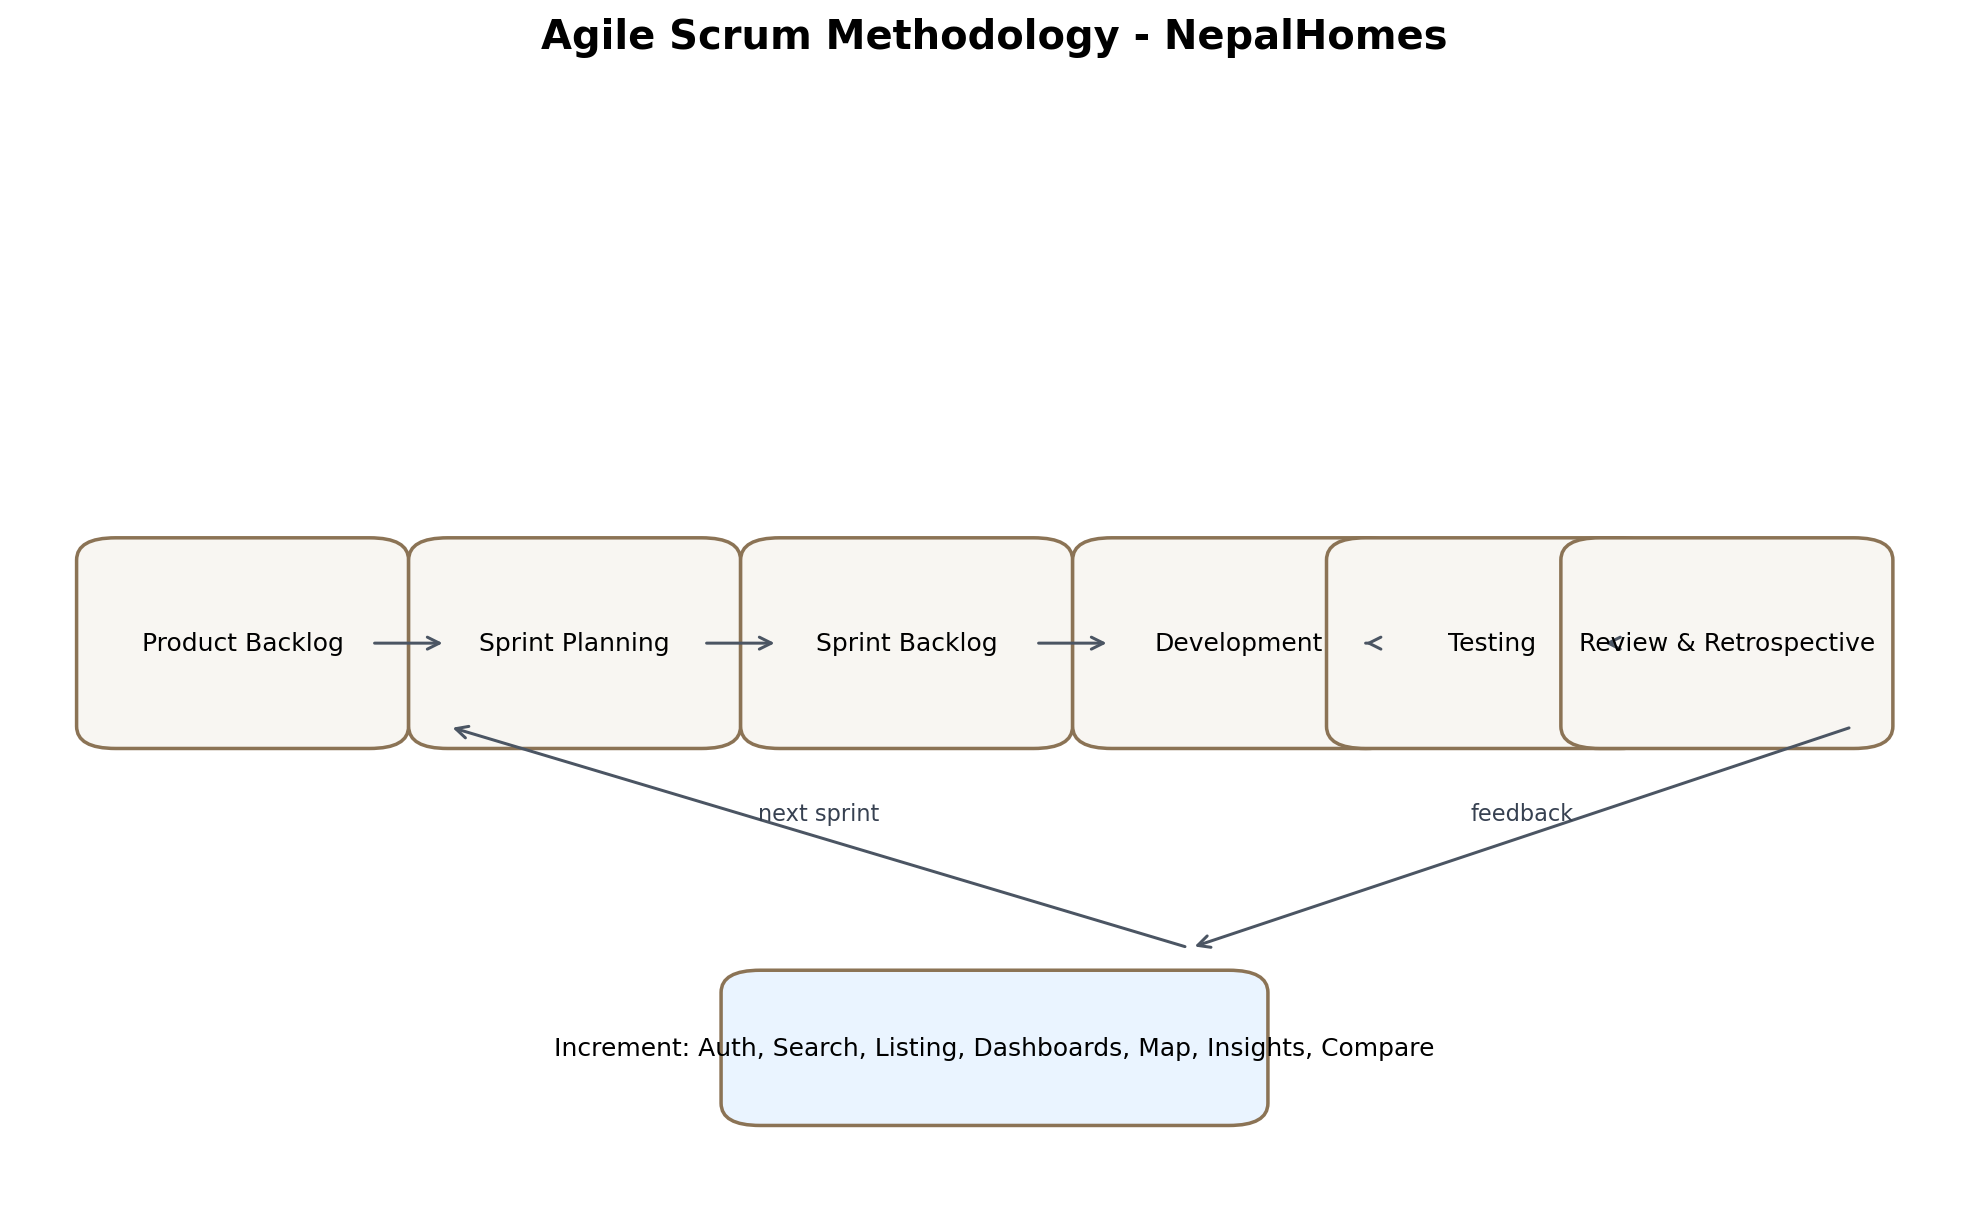
\includegraphics[width=0.95\textwidth]{figures/agile_scrum.png}
    \vspace{1cm}}}
  \caption{Agile Scrum Methodology}
  \label{fig:agile}
\end{figure}

\section{Organization of the Report}

This report is structured into several chapters, each discussing a specific area
of the NepalHomes project. The layout is as follows:

\begin{itemize}[leftmargin=2.5em]
  \item \textbf{Chapter 1: Introduction}\\
    Presents an overview of the project, including the problem statement,
    objectives, significance, limitations, development methodology, and report
    organisation.

  \item \textbf{Chapter 2: Background Study and Literature Review}\\
    Reviews existing real estate platforms, web development practices, and
    relevant academic literature, identifying the gaps that NepalHomes seeks
    to address.

  \item \textbf{Chapter 3: System Analysis}\\
    Provides a comprehensive overview of functional and non-functional
    requirements, feasibility studies, and UML diagrams modelling the system's
    behaviour and structure.

  \item \textbf{Chapter 4: System Design}\\
    Details the system architecture, class model, component design, and
    deployment structure of NepalHomes.

  \item \textbf{Chapter 5: Implementation and Testing}\\
    Describes the tools and technologies used, the implementation of each
    module, and the unit and system testing performed to verify correctness.

  \item \textbf{Chapter 6: Conclusion and Recommendations}\\
    Summarises findings, draws conclusions, and provides recommendations for
    future development.

  \item \textbf{References}\\
    Lists all sources cited throughout the report.

  \item \textbf{Appendices}\\
    Contains the Firestore data schema and application screenshots.
\end{itemize}

%============================================================
\chapter{Background Study and Literature Review}
%============================================================

\section{Background of the Study}

The global real estate industry has embraced digital transformation through
dedicated listing platforms such as Zillow, Rightmove, and 99acres, which
aggregate thousands of verified listings and provide structured search,
map-based discovery, and market analytics in a single interface. These platforms
have demonstrated that centralising property data and standardising listing
formats dramatically reduces the time and effort required for property discovery
and reduces information asymmetry between buyers and sellers.

In Nepal, real estate platforms remain nascent. Existing services such as
Hamrobazar and GharJagga offer basic listing aggregation but lack structured
address hierarchies aligned to Nepal's administrative divisions (Province,
District, Municipality, Ward), do not support Nepal-specific land measurement
units in search filters, and offer limited analytical tools for market
intelligence. The result is a marketplace that, while better than informal
channels, still requires significant manual effort to compare and evaluate
listings.

NepalHomes was conceived to fill this gap by building a platform purpose-designed
for the Nepali real estate market: using Nepal's seven-province and
seventy-seven-district administrative structure as the primary search dimension,
supporting aana, ropani, dhur, and bigha as first-class area units, and providing
market insights grounded in Nepali price data (NPR per aana). The project
demonstrates that a modern, full-featured real estate platform can be built using
only client-side technologies and serverless Firebase services, without the
infrastructure overhead of a dedicated backend server.

\section{Literature Review}

The design of NepalHomes draws on established research in web platform
architecture, user experience for property search, and the role of data
transparency in real estate markets.

Gefen and Straub \cite{gefen2004} demonstrated that perceived trust and
ease of use are the primary determinants of continued use for e-commerce
platforms. Their findings directly inform NepalHomes' admin approval workflow: by
requiring every seller-submitted listing to pass administrator review before
public visibility, the platform provides structural assurance to buyers that
listings are legitimate, increasing platform trust.

Nielsen's usability heuristics \cite{nielsen1994} emphasise the importance of
system status visibility and error prevention in user interface design. The
NepalHomes listing form implements these principles through a five-step wizard
with per-step validation (enforcing property type selection on Step~0, district
entry on Step~1, and title plus non-zero price on Step~2), immediate feedback
on validation failures, and a final review step before submission.

The effectiveness of map-based property search has been well documented.
Resnick and Varian \cite{resnick1997} established that geospatial context
significantly improves decision quality in information retrieval systems.
NepalHomes implements this through a full-screen Leaflet.js map centred on
Nepal, plotting all available properties as clickable markers that open detail
panels, enabling spatial reasoning in the property selection process.

From a data architecture perspective, the Firebase data persistence model
described by Moroney \cite{moroney2017} supports the NepalHomes storage
strategy. Cloud Firestore's document-collection model is used to store user
profiles, saved property lists, tour bookings, search alerts, and seller
submissions---with offline persistence enabled via \texttt{enablePersistence}
to ensure the platform remains usable under intermittent connectivity \cite{firebase2024}.

The existing literature identifies a gap specific to the Nepali market: no
published platform combines Nepal-specific administrative addressing, native
land units, role-based dashboards, and an embedded market analytics layer in a
single, freely accessible web application. NepalHomes addresses each of these
dimensions within a single codebase.

%============================================================
\chapter{System Analysis}
%============================================================

\section{System Analysis}

NepalHomes was developed iteratively using the Agile Scrum methodology. The
requirement analysis phase was conducted first, gathering and prioritising both
functional and non-functional requirements across all three user roles. The
resulting product backlog guided each development sprint, with the architecture,
data schema, and user interface evolving incrementally as features were built and
validated through end-to-end testing.

\subsection{Requirement Analysis}

Before commencing development, requirement gathering was carried out through
analysis of comparable real estate platforms, review of Nepal's land registration
and address conventions, and identification of the key workflows needed by buyers,
sellers, and administrators.

\subsubsection{Functional Requirements}

\begin{enumerate}[leftmargin=2.5em]
  \item \textbf{User Registration and Authentication:}
    The system must allow users to register with a first name, last name, email,
    phone number, password, and role selection (Buyer/Tenant or Seller/Owner).
    Login must use Firebase Email/Password authentication. Authenticated sessions
    must persist across page reloads via Firebase's built-in session management.

  \item \textbf{Role-Based Access Control:}
    Each role must be restricted to its appropriate pages. Buyer users must be
    redirected to \texttt{buyer-dashboard.html}; sellers to
    \texttt{seller-dashboard.html}; administrators to \texttt{admin.html}.
    Protected pages must redirect unauthenticated users to \texttt{login.html}
    with a \texttt{redirect} query parameter for post-login return.

  \item \textbf{Property Search and Filtering:}
    Users must be able to search properties by keyword, property type
    (House, Apartment, Land, Commercial), listing purpose (For Sale / For Rent),
    city, district, minimum and maximum price, and minimum bedroom count.
    The search must operate over both the 45 static demo properties and any
    Firestore-approved seller listings.

  \item \textbf{Property Detail View:}
    Each property must have a dedicated detail page displaying images with a
    navigation gallery, price, type, purpose, area (with unit), bedrooms,
    bathrooms, facing direction, road width, features, location, and seller
    contact information. A save button and tour booking form must be available
    on the detail page.

  \item \textbf{Saved Properties:}
    Authenticated buyers must be able to save and unsave properties using a heart
    icon. The saved list must be persisted to the user's Firestore document and
    must be accessible from the buyer dashboard.

  \item \textbf{Tour Booking:}
    Buyers must be able to book a property viewing by selecting a date and time
    from the property detail page. Bookings must be stored in Firestore and
    cancellable from the buyer dashboard.

  \item \textbf{Search Alerts:}
    Buyers must be able to create named search alerts with a query description
    and a notification frequency (Daily, Weekly, Monthly). Alerts must be
    stored in Firestore and manageable from the buyer dashboard.

  \item \textbf{Property Listing (Seller):}
    Authenticated sellers must be able to submit a property through a five-step
    guided form capturing: property type and purpose; province, district,
    municipality, ward, tole, and city; title, price, area, bedrooms, bathrooms,
    facing, road width, amenities, and description; photos (placeholder); and a
    review screen. Submissions must be saved to Firestore with status
    \texttt{pending} and associated with the seller's user ID.

  \item \textbf{Seller Dashboard:}
    Sellers must be able to view all their submitted properties with their current
    approval status (pending/approved/rejected), delete listings, view a mock
    inquiries list, and view a Chart.js analytics panel with weekly view counts.

  \item \textbf{Admin Approval Workflow:}
    Administrators must be able to view all submitted properties, approve or
    reject pending listings, and re-set approved or rejected listings back to
    pending. The admin dashboard must display counts of total submissions,
    pending reviews, approved listings, and registered users.

  \item \textbf{Interactive Map View:}
    The map page must display a full-screen Leaflet.js map centred on Nepal
    with markers for the static 	exttt{PROPERTIES} dataset. Clicking a marker
    must open a popup with the property image, title, price, and a link to the
    detail page. The map supports status/type pill filters (All, Sale, Rent,
    House, Apartment, Land).

  \item \textbf{Property Comparison:}
    Users must be able to select up to three properties from a search-enabled
    picker and compare them side by side in a table showing price, area, beds,
    baths, location, type, purpose, and features. The comparison must highlight
    winner values (lowest price, largest area, most bedrooms) with coloured
    badges.

  \item \textbf{Market Insights:}
    The insights page must display: KPI cards for average price per aana in
    Kathmandu and Pokhara, active listings count, and average days on market;
    a Chart.js line chart of price trends for three cities (2026 monthly data);
    a bar chart of new listings versus sales; a doughnut chart of listings by
    property type; a ranked list of top locations with progress bars; and a
    narrative market summary section.
\end{enumerate}

\subsubsection{Non-Functional Requirements}

\begin{itemize}[leftmargin=2.5em]
  \item \textbf{Performance:}
    The platform must load all major pages without a build step or bundler.
    Using static HTML files served directly from the file system or a CDN ensures
    sub-second initial load. JavaScript is loaded as separate script tags, keeping
    individual file sizes manageable.

  \item \textbf{Usability:}
    The interface must use a consistent design system (CSS custom properties,
    shared utility classes) across all pages. Navigation must be available via a
    persistent top navbar with a hamburger menu on mobile, and user actions must
    require minimal clicks to complete common tasks.

  \item \textbf{Security:}
    All authenticated pages must verify the Firebase auth state before rendering
    content. Role guards must prevent buyers from accessing the seller dashboard
    and vice versa. Firestore security rules must restrict document access to
    authenticated users.

  \item \textbf{Reliability:}
    Firestore offline persistence must be enabled with \texttt{synchronizeTabs:
    true} so that cached data remains accessible during brief connectivity
    interruptions. The platform must handle missing Firestore documents
    gracefully without crashing.

  \item \textbf{Responsiveness:}
    The layout must adapt correctly to desktop (1280\,px+), tablet (768\,px),
    and mobile (375\,px) screen sizes using CSS media queries. The navbar must
    collapse to a hamburger menu on screens narrower than 768\,px.

  \item \textbf{Accessibility:}
    Buttons must include \texttt{title} attributes for screen reader support.
    Form labels must be explicitly associated with their input fields.
    Interactive elements must have sufficient colour contrast against backgrounds.

  \item \textbf{Scalability:}
    The Firestore backend scales automatically with the volume of listings and
    users, requiring no manual infrastructure management as the platform grows.
    The static frontend can be served from any web server or CDN without
    modification.
\end{itemize}

\subsection{Feasibility Analysis}

A feasibility study was conducted across four dimensions before commencing
development.

\subsubsection{Technical Feasibility Study}

NepalHomes is built entirely on freely available, well-documented technologies.
HTML5, CSS3, and vanilla JavaScript require no proprietary tools and run in
every modern browser. Firebase Authentication and Cloud Firestore are production-
grade Google services with generous free-tier quotas (50,000 Firestore reads
per day, 20,000 writes per day) sufficient to support a student project and
initial launch. Leaflet.js and Chart.js are mature, well-supported open-source
libraries available via CDN. All technical dependencies are within the existing
skill set of a BIT graduate.

\subsubsection{Operational Feasibility Study}

The platform requires only a modern web browser on any device, making it
accessible to property seekers across Nepal regardless of hardware. The intuitive
UI with step-by-step guided forms, inline validation messages, and role-specific
dashboards minimises the training required for new users. The admin approval
workflow is straightforward and does not require any specialised database tools.

\subsubsection{Economic Feasibility Study}

All development tools are free and open-source. Firebase Hosting, available at
no cost on the Spark plan, can serve the static HTML files globally. The Firebase
free tier accommodates development and initial production use without cost. No
additional hardware or software licences are required.

\subsubsection{Schedule Feasibility Study}

The project was planned with clear phases assigned to each development sprint,
ensuring timely completion within the academic semester.

\begin{table}[H]
\centering
\caption{Development Schedule of NepalHomes}
\label{tab:schedule}
\begin{tabular}{@{}lc@{}}
\toprule
\textbf{Task Name} & \textbf{Duration} \\
\midrule
Planning and Requirement Analysis       & 2 weeks \\
UI/UX Design and CSS Design System      & 2 weeks \\
Firebase Setup and Authentication       & 1 week  \\
Core Pages (Index, Search, Property)    & 4 weeks \\
Dashboards and Admin Panel              & 3 weeks \\
Map, Insights, and Comparison Tools     & 3 weeks \\
Testing, Bug Fixing, and Polish         & 3 weeks \\
\bottomrule
\end{tabular}
\end{table}

\begin{figure}[H]
  \begin{flushleft}
    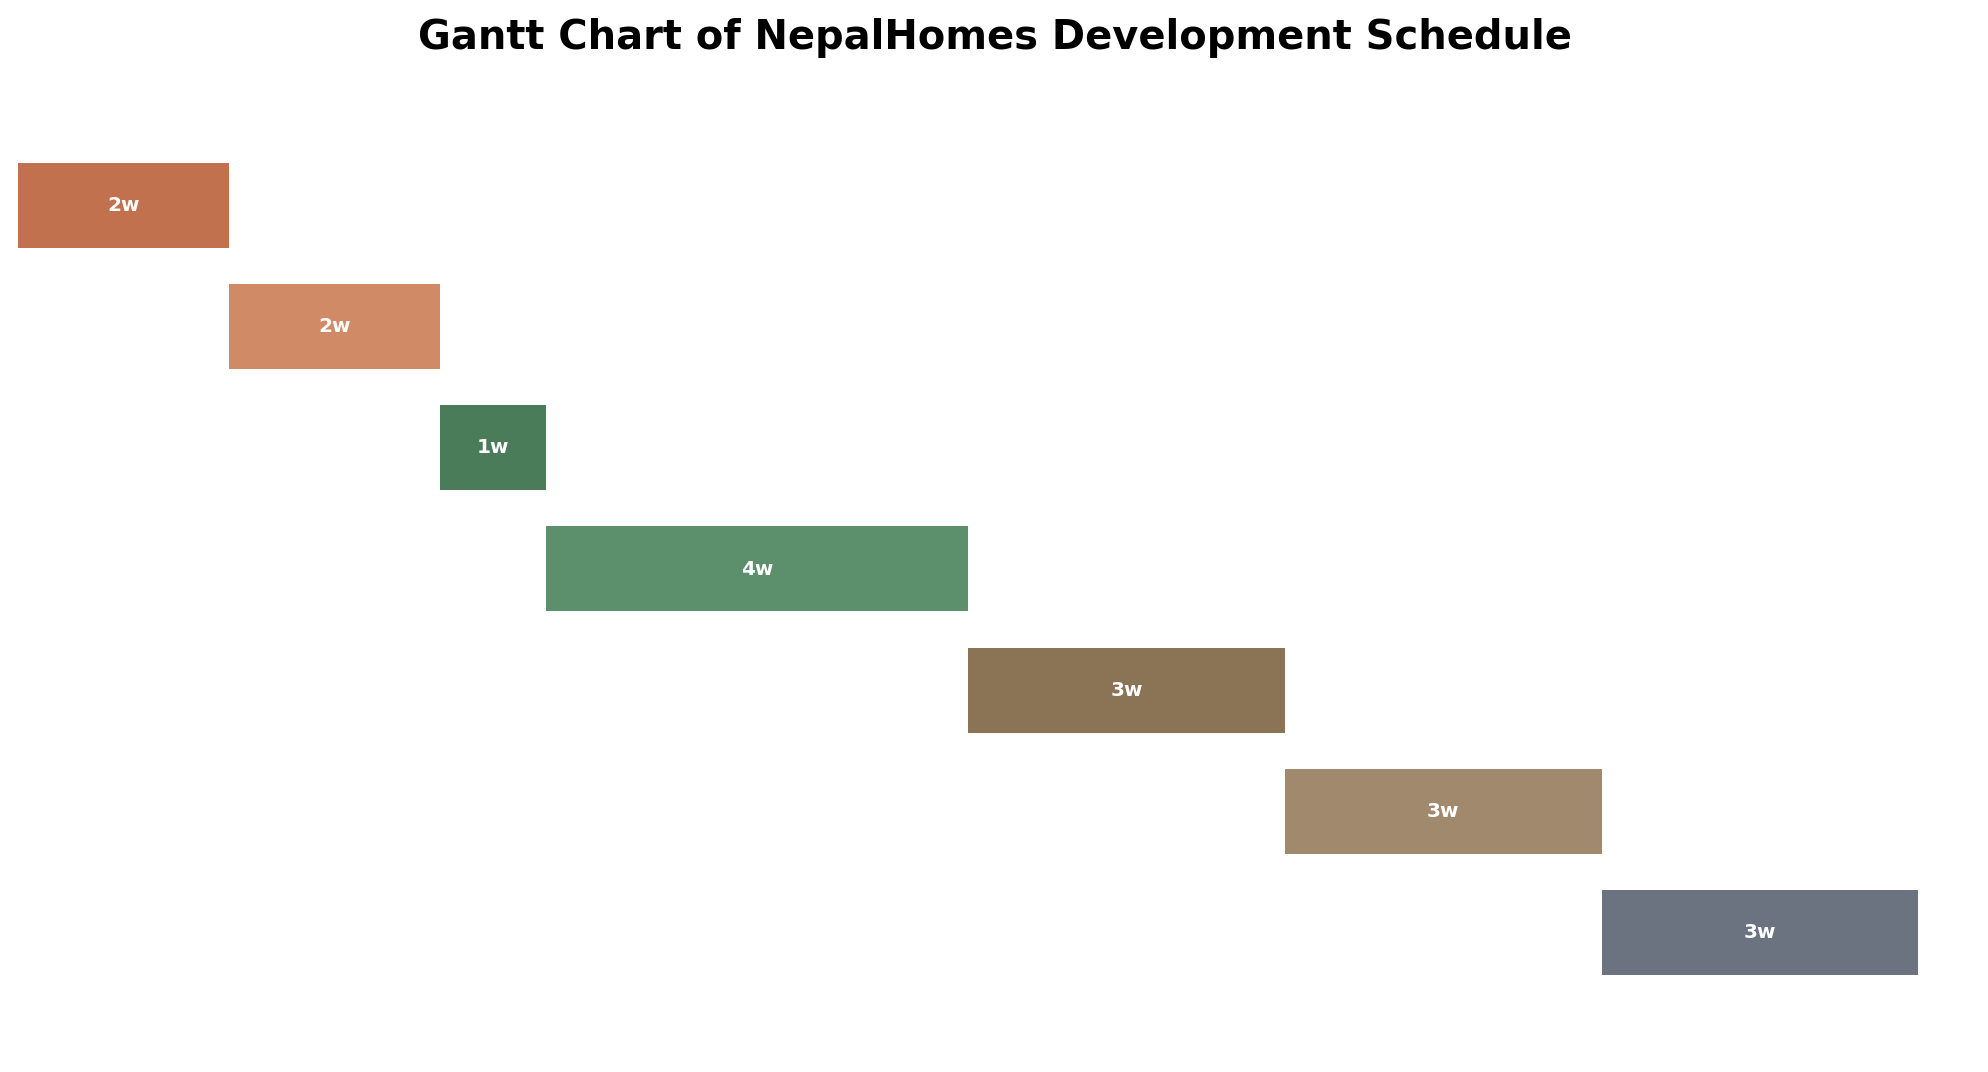
\includegraphics[width=0.95\textwidth]{figures/gantt_chart.png}
  \end{flushleft}
  \caption{Gantt Chart of NepalHomes Development Schedule}
  \label{fig:gantt}
\end{figure}

\subsection{System Modeling}

\subsubsection{Use Case Diagram}

The primary actors in NepalHomes are Guest (unauthenticated user), Buyer/Tenant,
Seller/Owner, and Administrator. Key use cases include: Register Account,
Login/Logout, Search Properties, View Property Detail, Save Property, Book
Viewing Tour, Create Search Alert, List Property, View Seller Dashboard,
Approve/Reject Listing, and View Admin Dashboard.

\begin{figure}[H]
  \centering
  \fbox{\parbox{0.82\textwidth}{\centering\vspace{1cm}
    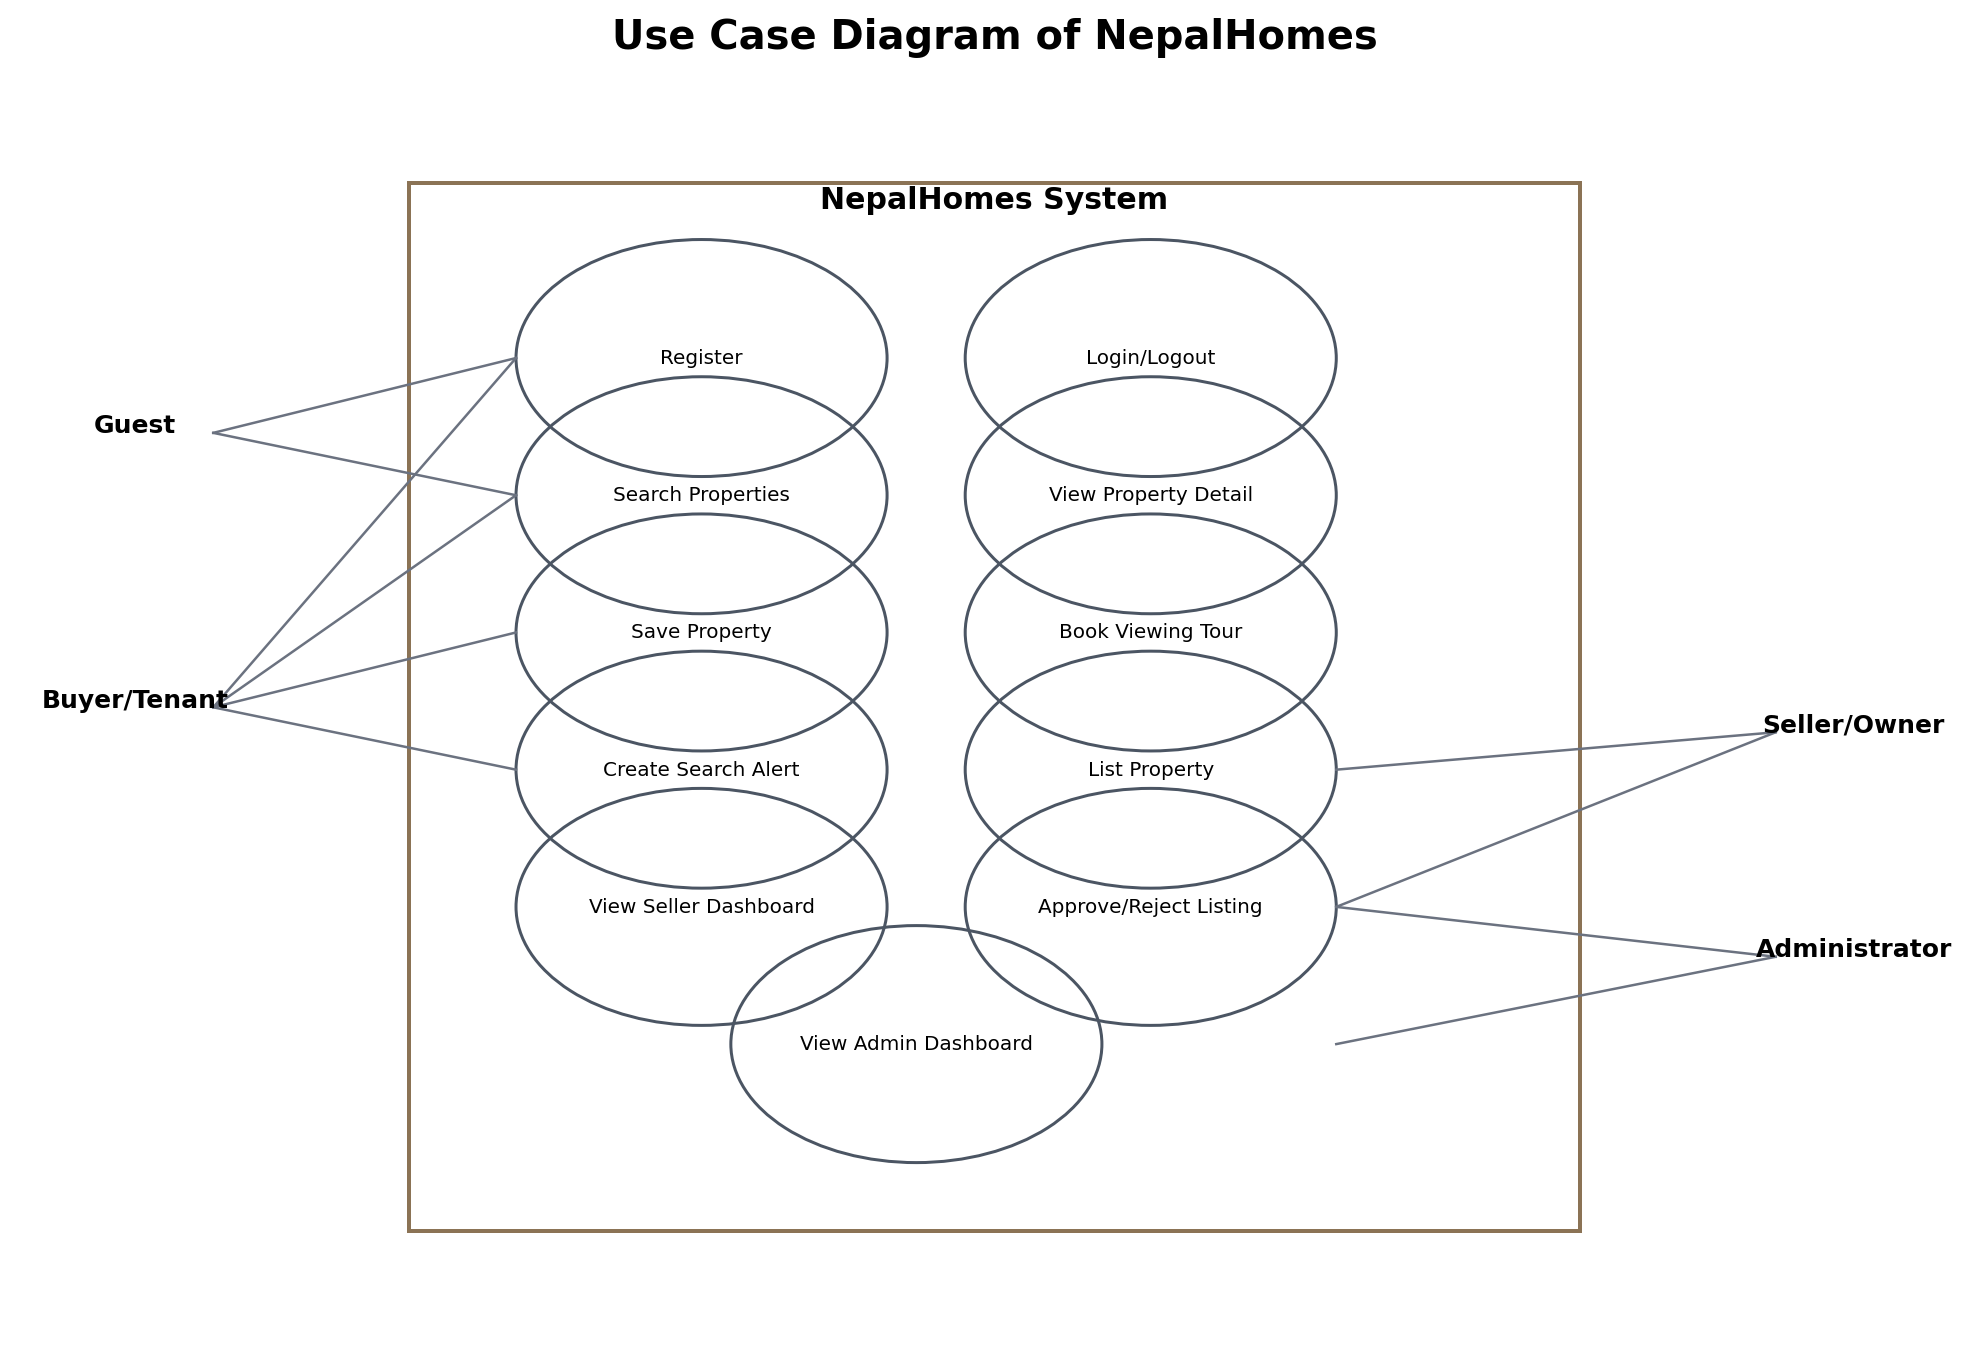
\includegraphics[width=0.8\textwidth]{figures/use_case_diagram.png}
    \vspace{1cm}}}
  \caption{Use Case Diagram of NepalHomes}
  \label{fig:usecase}
\end{figure}

\subsubsection{Class Diagram}

Primary classes include: User (with specialisations Buyer, Seller, Admin),
Property, SavedList, Tour, SearchAlert, and AdminAction. Property is the central
entity, referenced by SavedList entries, Tour records, and AdminAction events.

\begin{figure}[H]
  \centering
  \fbox{\parbox{1\textwidth}{\centering\vspace{1cm}
    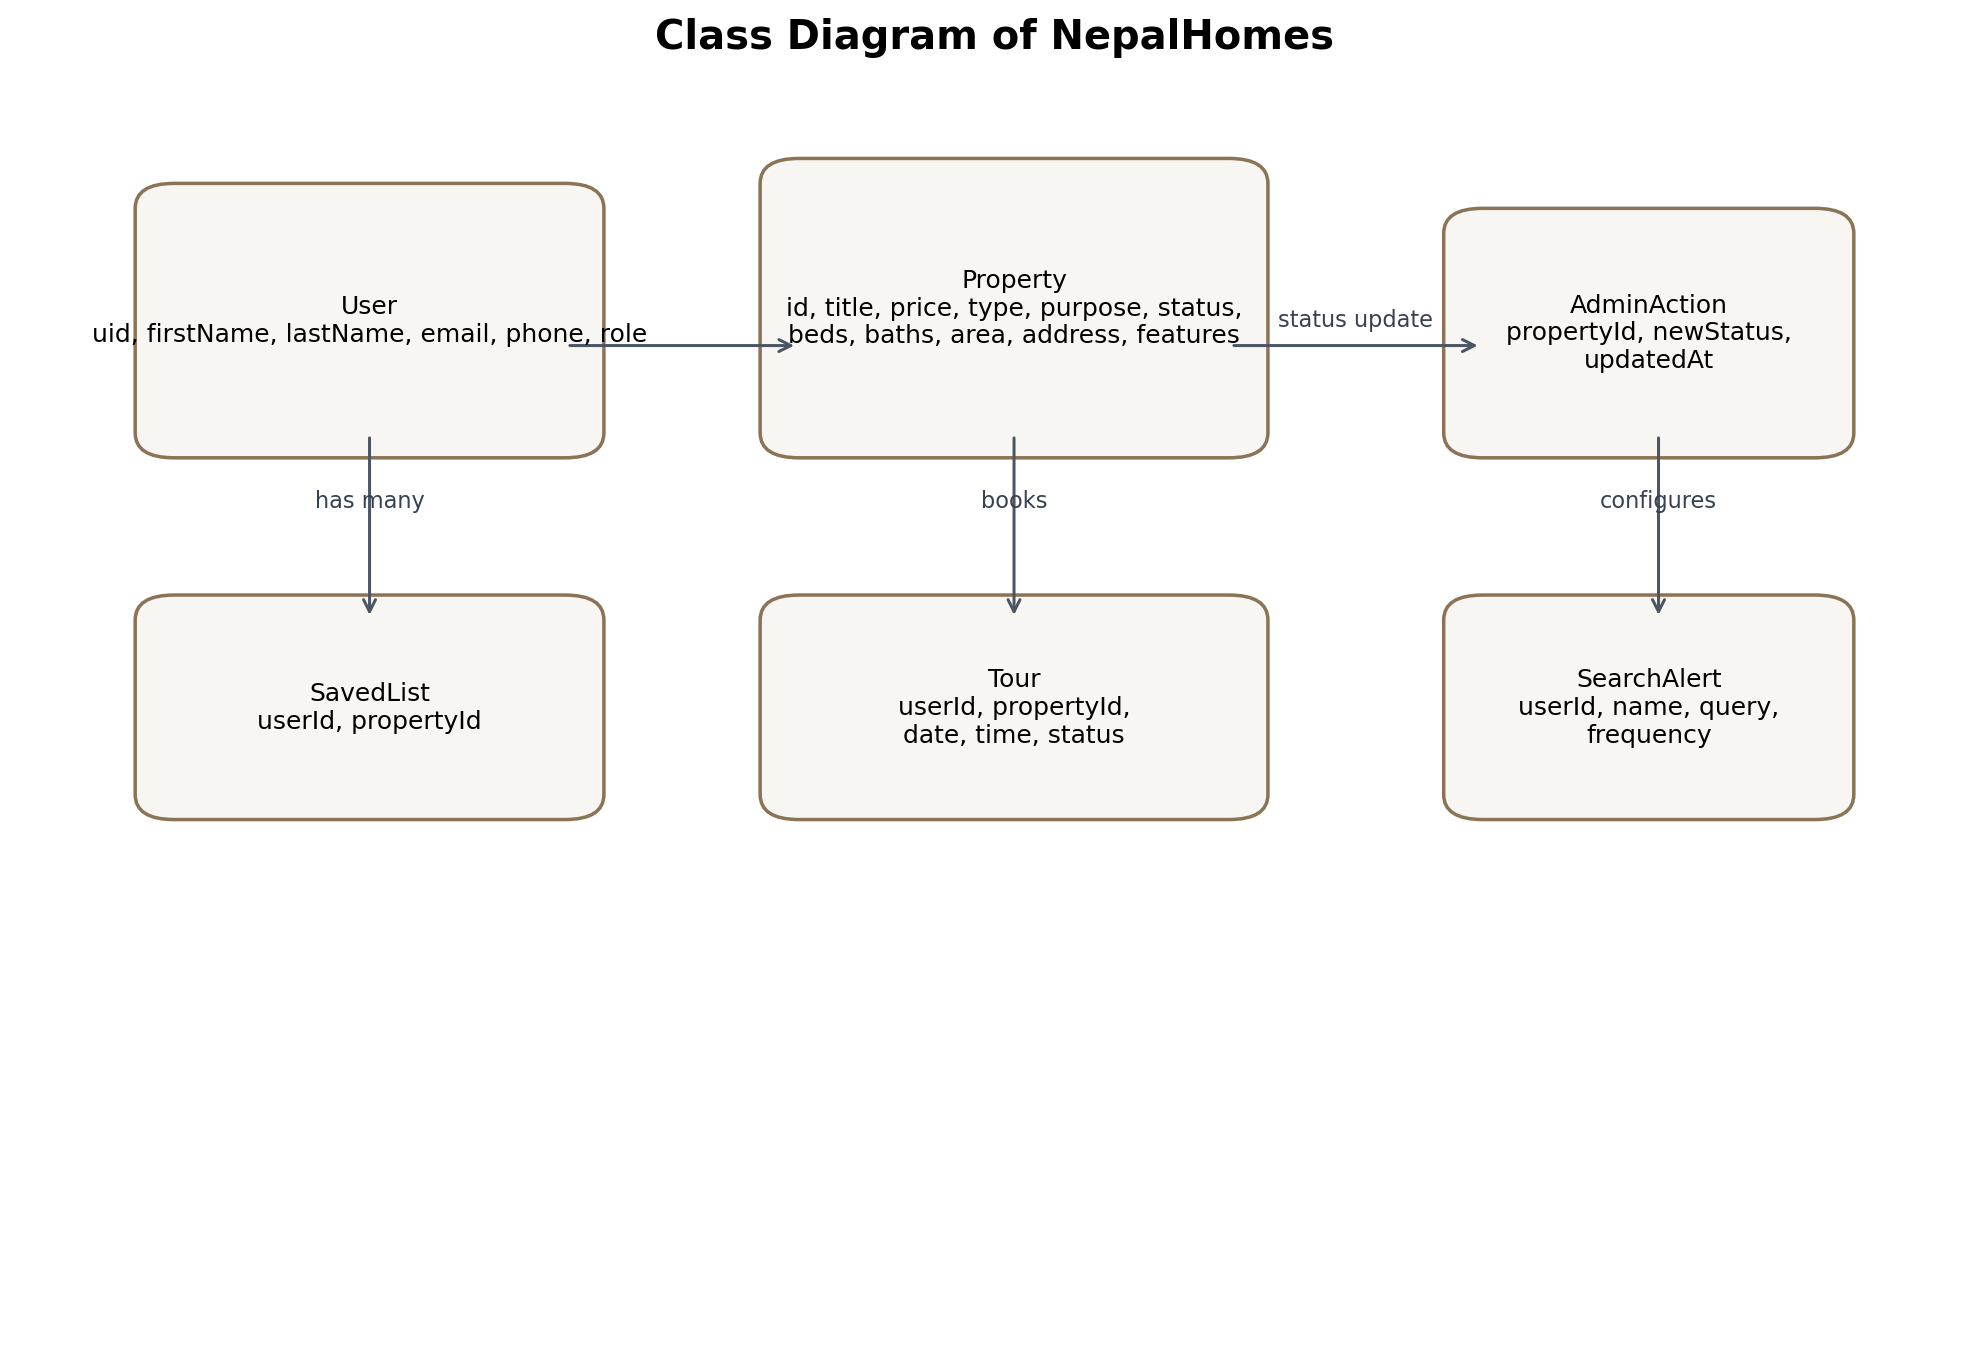
\includegraphics[width=0.95\textwidth]{figures/class_diagram.png}
    \vspace{1cm}}}
  \caption{Class Diagram of NepalHomes}
  \label{fig:class}
\end{figure}

\subsection{Dynamic Modeling using State and Sequence Diagrams}

\subsubsection{Sequence Diagram}

The sequence diagram for the property listing and approval flow illustrates the
following interactions: the Seller completes the five-step listing form and
submits; the frontend writes a \texttt{properties} document to Firestore with
\texttt{status: pending}; the Admin opens \texttt{admin.html}, which queries all
Firestore properties; the Admin clicks Approve; the frontend updates the document
\texttt{status} field to \texttt{approved}; approved properties become visible in
the public search results.

\begin{figure}[H]
  \centering
  \fbox{\parbox{1\textwidth}{\centering\vspace{1cm}
    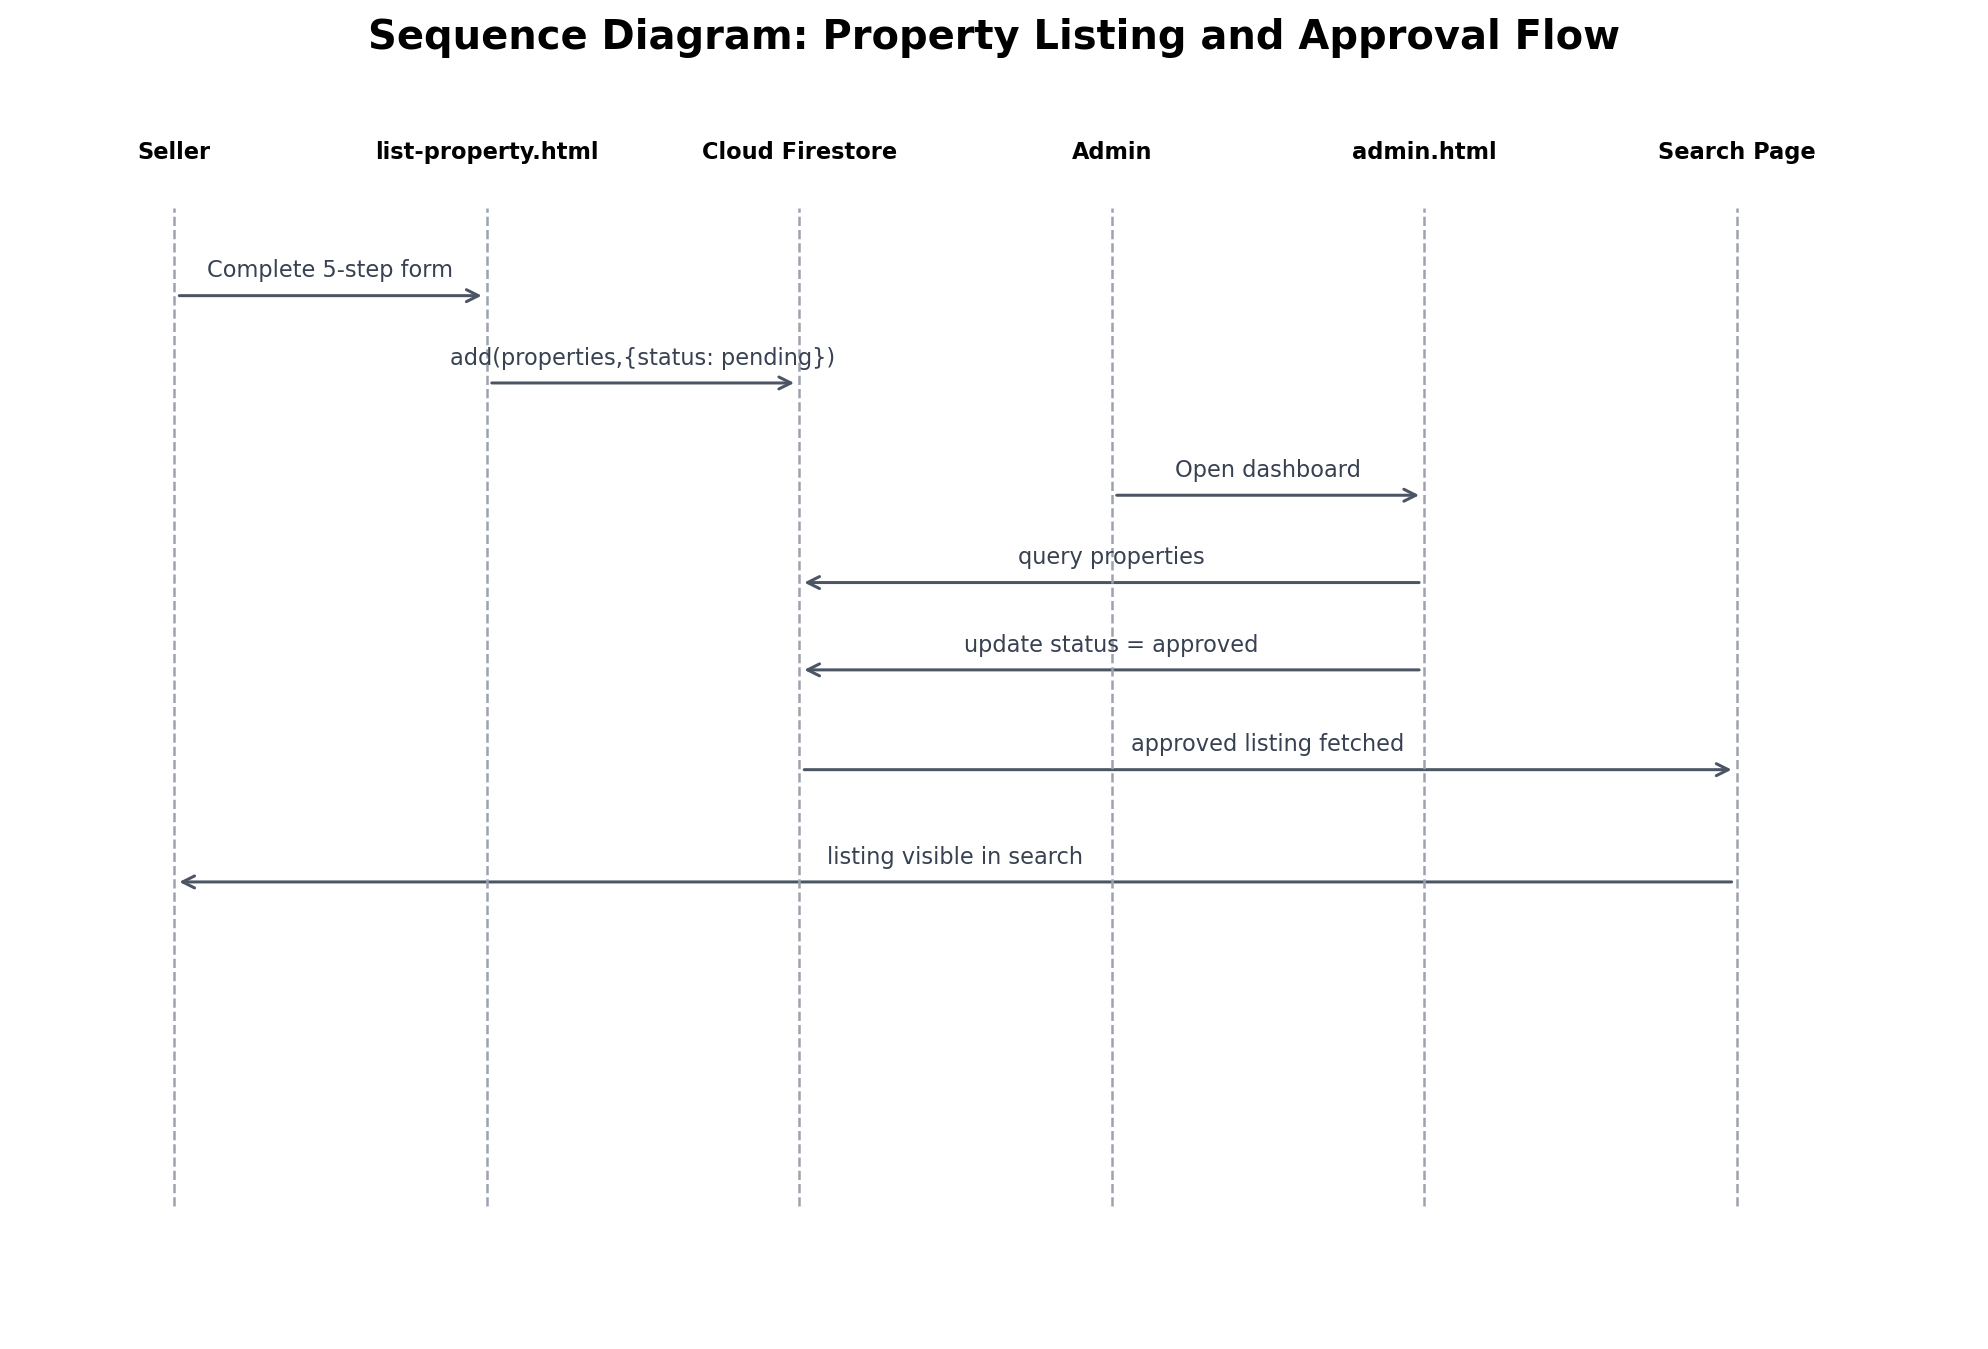
\includegraphics[width=0.95\textwidth]{figures/sequence_diagram.png}
    \vspace{1cm}}}
  \caption{Sequence Diagram: Property Listing and Approval Flow}
  \label{fig:sequence}
\end{figure}

\subsection{Process Modeling using Activity Diagrams}

\subsubsection{Activity Diagram}

The activity diagram for the buyer property search and save workflow shows:
the User opens the Search page; enters keywords and applies filters; the system
merges static properties and approved Firestore listings and renders matching
cards; the User clicks a card to view the property detail page; the User clicks
the heart icon to save the property; if not logged in, the system redirects to
the login page; upon login, the save is persisted to the user's Firestore
document; the saved property appears in the Buyer Dashboard under Saved Properties.

\begin{figure}[H]
  \centering
  \fbox{\parbox{1\textwidth}{\centering\vspace{1cm}
    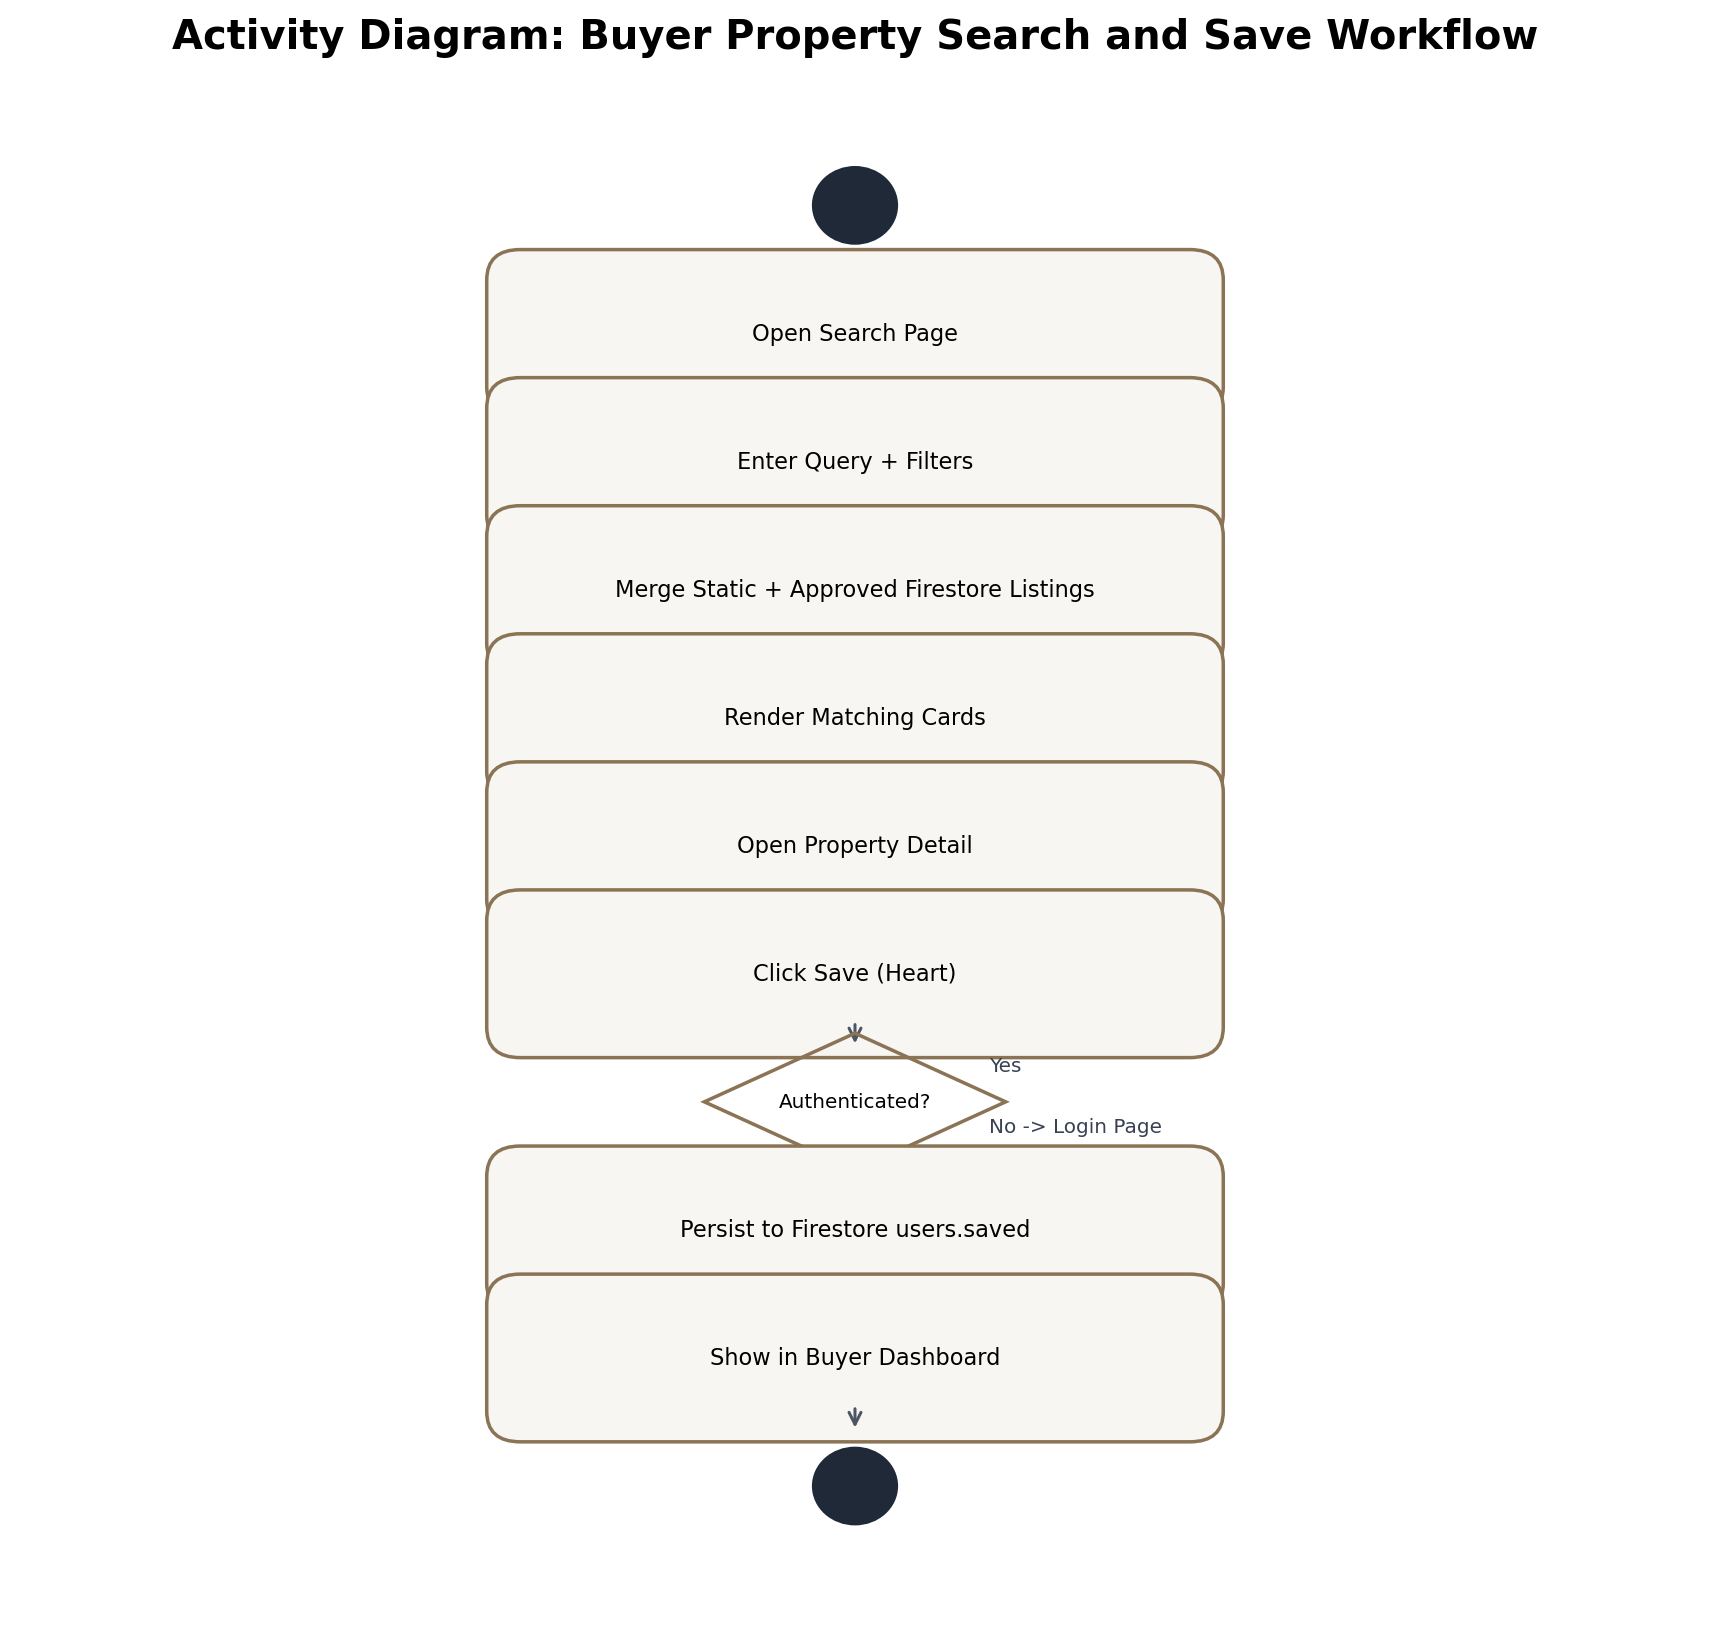
\includegraphics[width=0.9\textwidth]{figures/activity_diagram.png}
    \vspace{1cm}}}
  \caption{Activity Diagram: Buyer Property Search and Save Workflow}
  \label{fig:activity}
\end{figure}

%============================================================
\chapter{System Design}
%============================================================

System design transforms the requirements identified during analysis into a
concrete blueprint for the NepalHomes implementation. It defines the data model,
component architecture, and deployment topology of the system.

\section{Refinement of Classes and Objects}

The following classes form the backbone of the NepalHomes data model, represented
in Cloud Firestore as document collections:

\begin{itemize}[leftmargin=2.5em]
  \item \textbf{User:} Represents all registered platform users. Attributes:
    \texttt{uid} (Firebase Auth UID), \texttt{firstName}, \texttt{lastName},
    \texttt{email}, \texttt{phone}, \texttt{role} (buyer/seller/admin),
    \texttt{saved} (array of property IDs), \texttt{tours} (array of Tour
    objects), \texttt{alerts} (array of SearchAlert objects),
    \texttt{createdAt}.

  \item \textbf{Property:} Represents a real estate listing. For static demo
    properties, stored in the JavaScript \texttt{PROPERTIES} array with numeric
    IDs. For seller-submitted properties, stored in the Firestore
    \texttt{properties} collection with auto-generated string document IDs.
    Attributes: \texttt{id}, \texttt{title}, \texttt{price}, \texttt{type}
    (house/apartment/land/commercial), \texttt{purpose} (for\_sale/for\_rent),
    \texttt{status} (pending/approved/rejected), \texttt{beds}, \texttt{baths},
    \texttt{area}, \texttt{areaUnit}, \texttt{province}, \texttt{district},
    \texttt{municipality}, \texttt{ward}, \texttt{tole}, \texttt{city},
    \texttt{description}, \texttt{features}, \texttt{facing}, \texttt{road},
    \texttt{image}, \texttt{sellerId}, \texttt{sellerName}, \texttt{sellerPhone},
    \texttt{createdAt}.

  \item \textbf{Tour:} Embedded in the User document's \texttt{tours} array.
    Attributes: \texttt{id} (timestamp), \texttt{propertyId}, \texttt{date},
    \texttt{time}, \texttt{status} (pending/confirmed).

  \item \textbf{SearchAlert:} Embedded in the User document's \texttt{alerts}
    array. Attributes: \texttt{id} (timestamp), \texttt{name}, \texttt{query},
    \texttt{frequency} (Daily/Weekly/Monthly), \texttt{createdAt}.

  \item \textbf{AdminAction:} Represented implicitly by the \texttt{status}
    field of each Property document. When an administrator calls
    \texttt{changeStatus(firestoreId, newStatus)}, the Firestore document is
    updated and the in-memory cache is synchronised, updating all rendered
    dashboard tables without a page reload.
\end{itemize}

\begin{figure}[H]
  \centering
  \fbox{\parbox{0.82\textwidth}{\centering\vspace{1cm}
    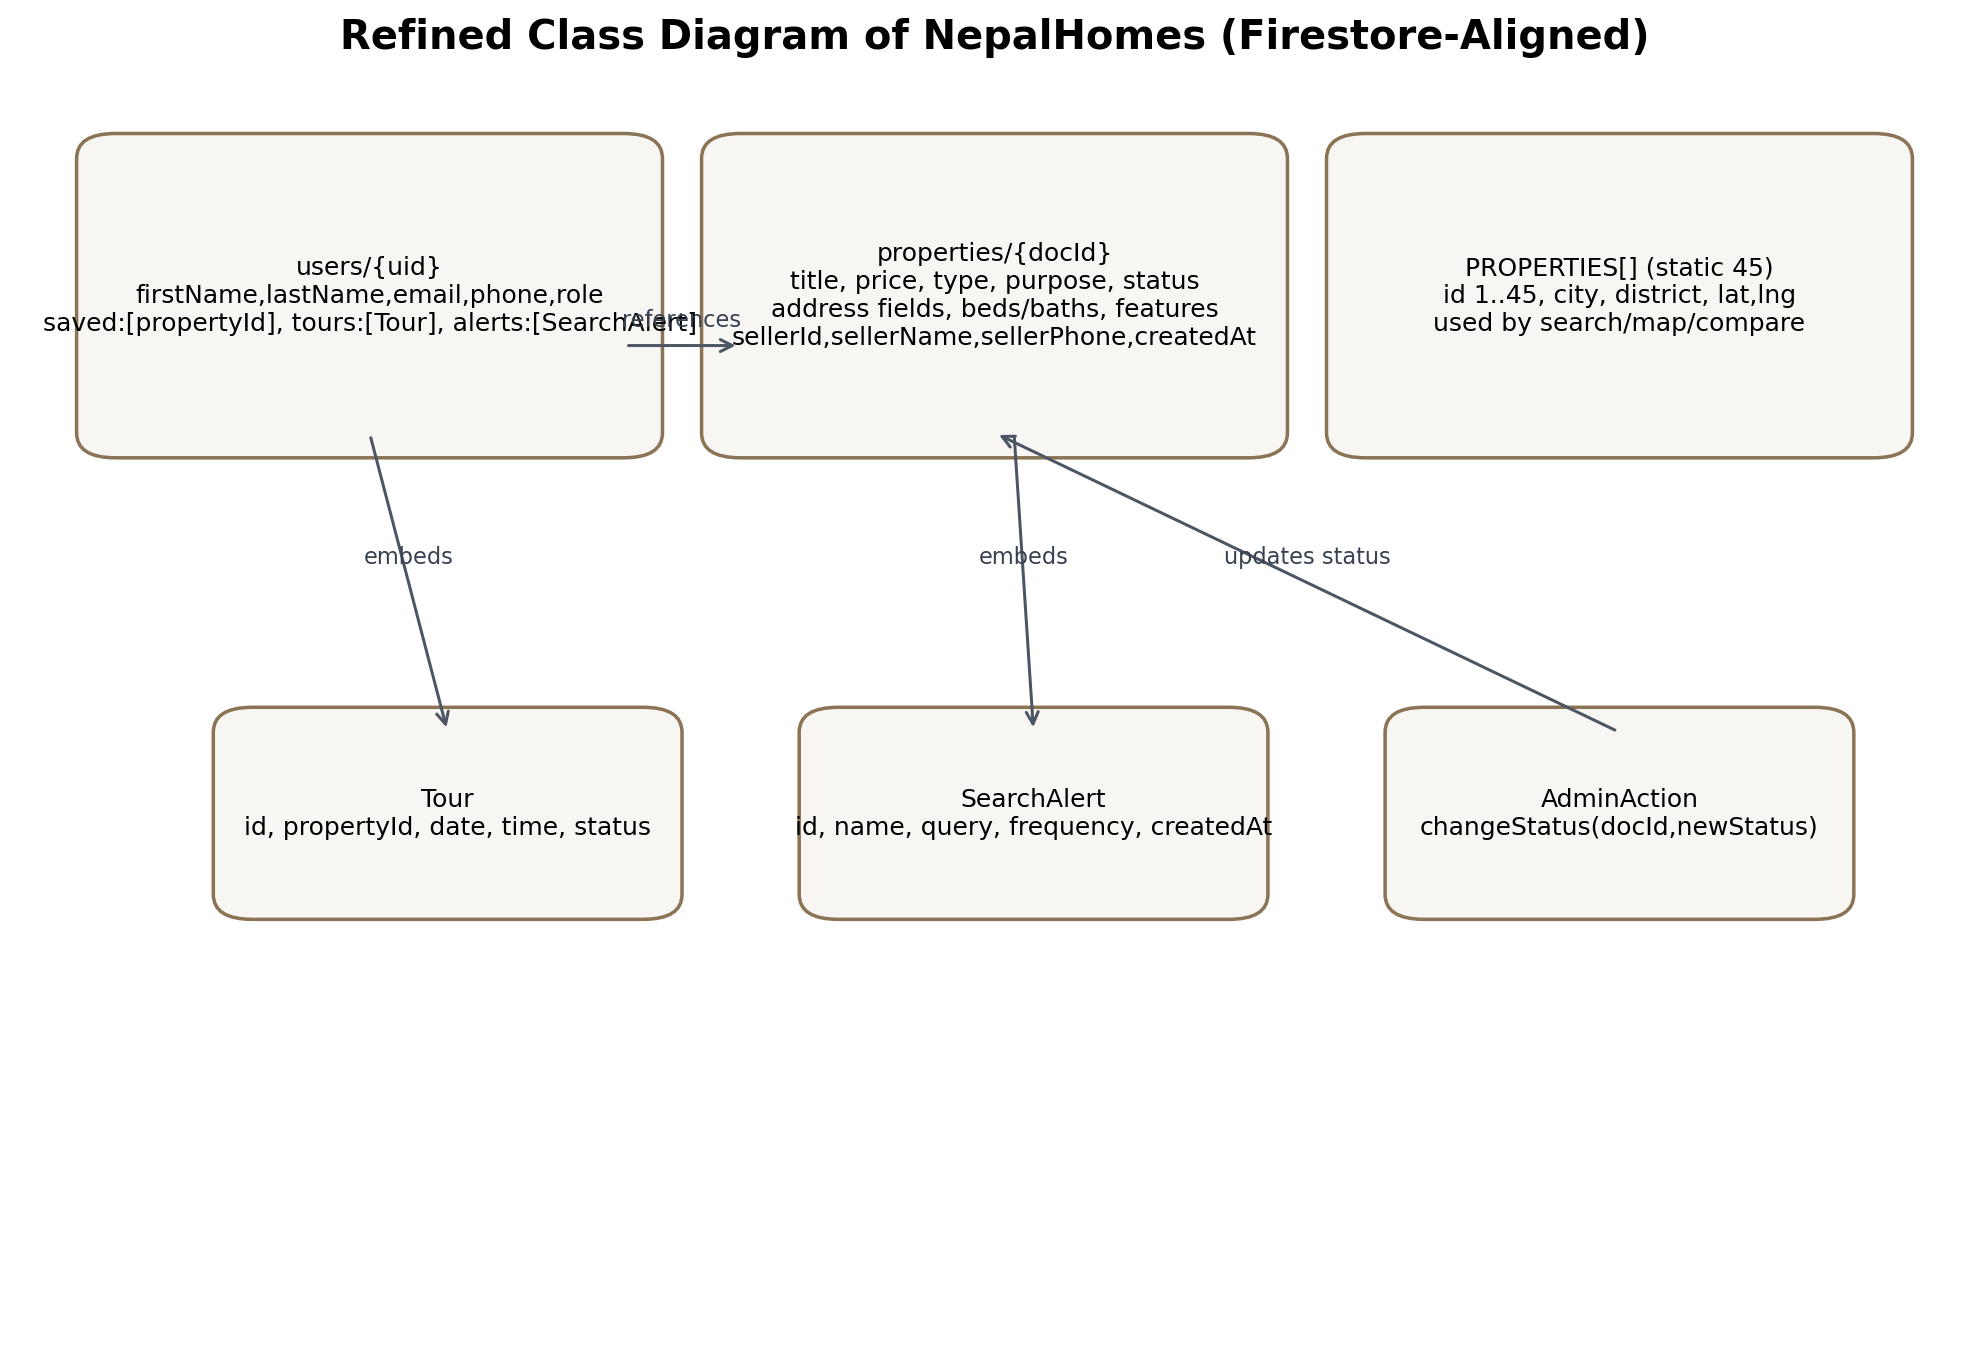
\includegraphics[width=0.85\textwidth]{figures/refined_class_diagram.png}
    \vspace{1cm}}}
  \caption{Refined Class Diagram of NepalHomes}
  \label{fig:refined-class}
\end{figure}

\section{Component Diagram}

The Component Diagram illustrates the relationships between the major components
of the NepalHomes system.

\noindent\textbf{i.\ Static Frontend (HTML/CSS/JS Pages):}

The frontend consists of twelve static HTML pages, each loaded independently.
Shared functionality is provided by four JavaScript modules loaded as
\texttt{<script>} tags: \texttt{firebase.js} (Firebase initialisation),
\texttt{auth.js} (authentication, saved properties, tours, alerts),
\texttt{data.js} (static PROPERTIES array, city list, formatters,
\texttt{propertyCardHTML} generator), and \texttt{layout.js} (navbar and footer
rendering). Pages include: \texttt{index.html}, \texttt{search.html},
\texttt{property.html}, \texttt{map.html}, \texttt{compare.html},
\texttt{insights.html}, \texttt{list-property.html},
\texttt{buyer-dashboard.html}, \texttt{seller-dashboard.html},
\texttt{admin.html}, \texttt{login.html}, and \texttt{register.html}.

\noindent\textbf{ii.\ Firebase Authentication:}

Firebase Authentication (compat SDK v10.12.5) provides email and password-based
user registration and login. The \texttt{auth.onAuthStateChanged} listener in
\texttt{auth.js} fires on every page load and populates the \texttt{\_currentUser}
cache with merged Firebase Auth and Firestore user data. Role-based redirects and
page guards are implemented using \texttt{onAuthReady()} and
\texttt{requireAuth()} helper functions.

\noindent\textbf{iii.\ Cloud Firestore:}

Cloud Firestore stores two top-level collections: \texttt{users} (one document
per registered user, keyed by Firebase Auth UID) and \texttt{properties} (one
document per seller submission, with auto-generated string IDs). Offline
persistence is enabled via \texttt{db.enablePersistence(\{synchronizeTabs:
true\})} to support tab synchronisation and brief connectivity interruptions.

\noindent\textbf{iv.\ Leaflet.js Map Engine:}

The \texttt{map.html} page loads Leaflet.js from CDN and renders a full-screen
map initialised at Nepal's geographic centroid (28.3949\textdegree N,
84.124\textdegree E, zoom 7). Each of the 45 static demo properties is plotted
as a custom marker rendered by \texttt{propertyCardHTML(p)} embedded in a Leaflet
popup. Status/type pill filters control which property markers are displayed.

\noindent\textbf{v.\ Chart.js Visualisation Engine:}

The \texttt{insights.html} and \texttt{seller-dashboard.html} pages load Chart.js
v4.4.0 from CDN. The insights page renders four charts: a multi-line price trend
chart (KTM/PKR/Lalitpur), a grouped bar chart (new listings vs.\ sold), a
doughnut chart (listings by type), and a ranked location list with HTML progress
bars. The seller dashboard renders a weekly views bar chart using mock data.

\noindent\textbf{vi.\ Static Data Layer:}

\texttt{data.js} provides 45 curated demo properties in the \texttt{PROPERTIES}
array (numeric IDs 1--45), the \texttt{CITIES} array, price formatting utilities,
and the \texttt{propertyCardHTML(p)} function that generates consistent property
card HTML for use across the search, compare, and map pages.

\begin{figure}[H]
  \centering
  \fbox{\parbox{0.82\textwidth}{\centering\vspace{1cm}
    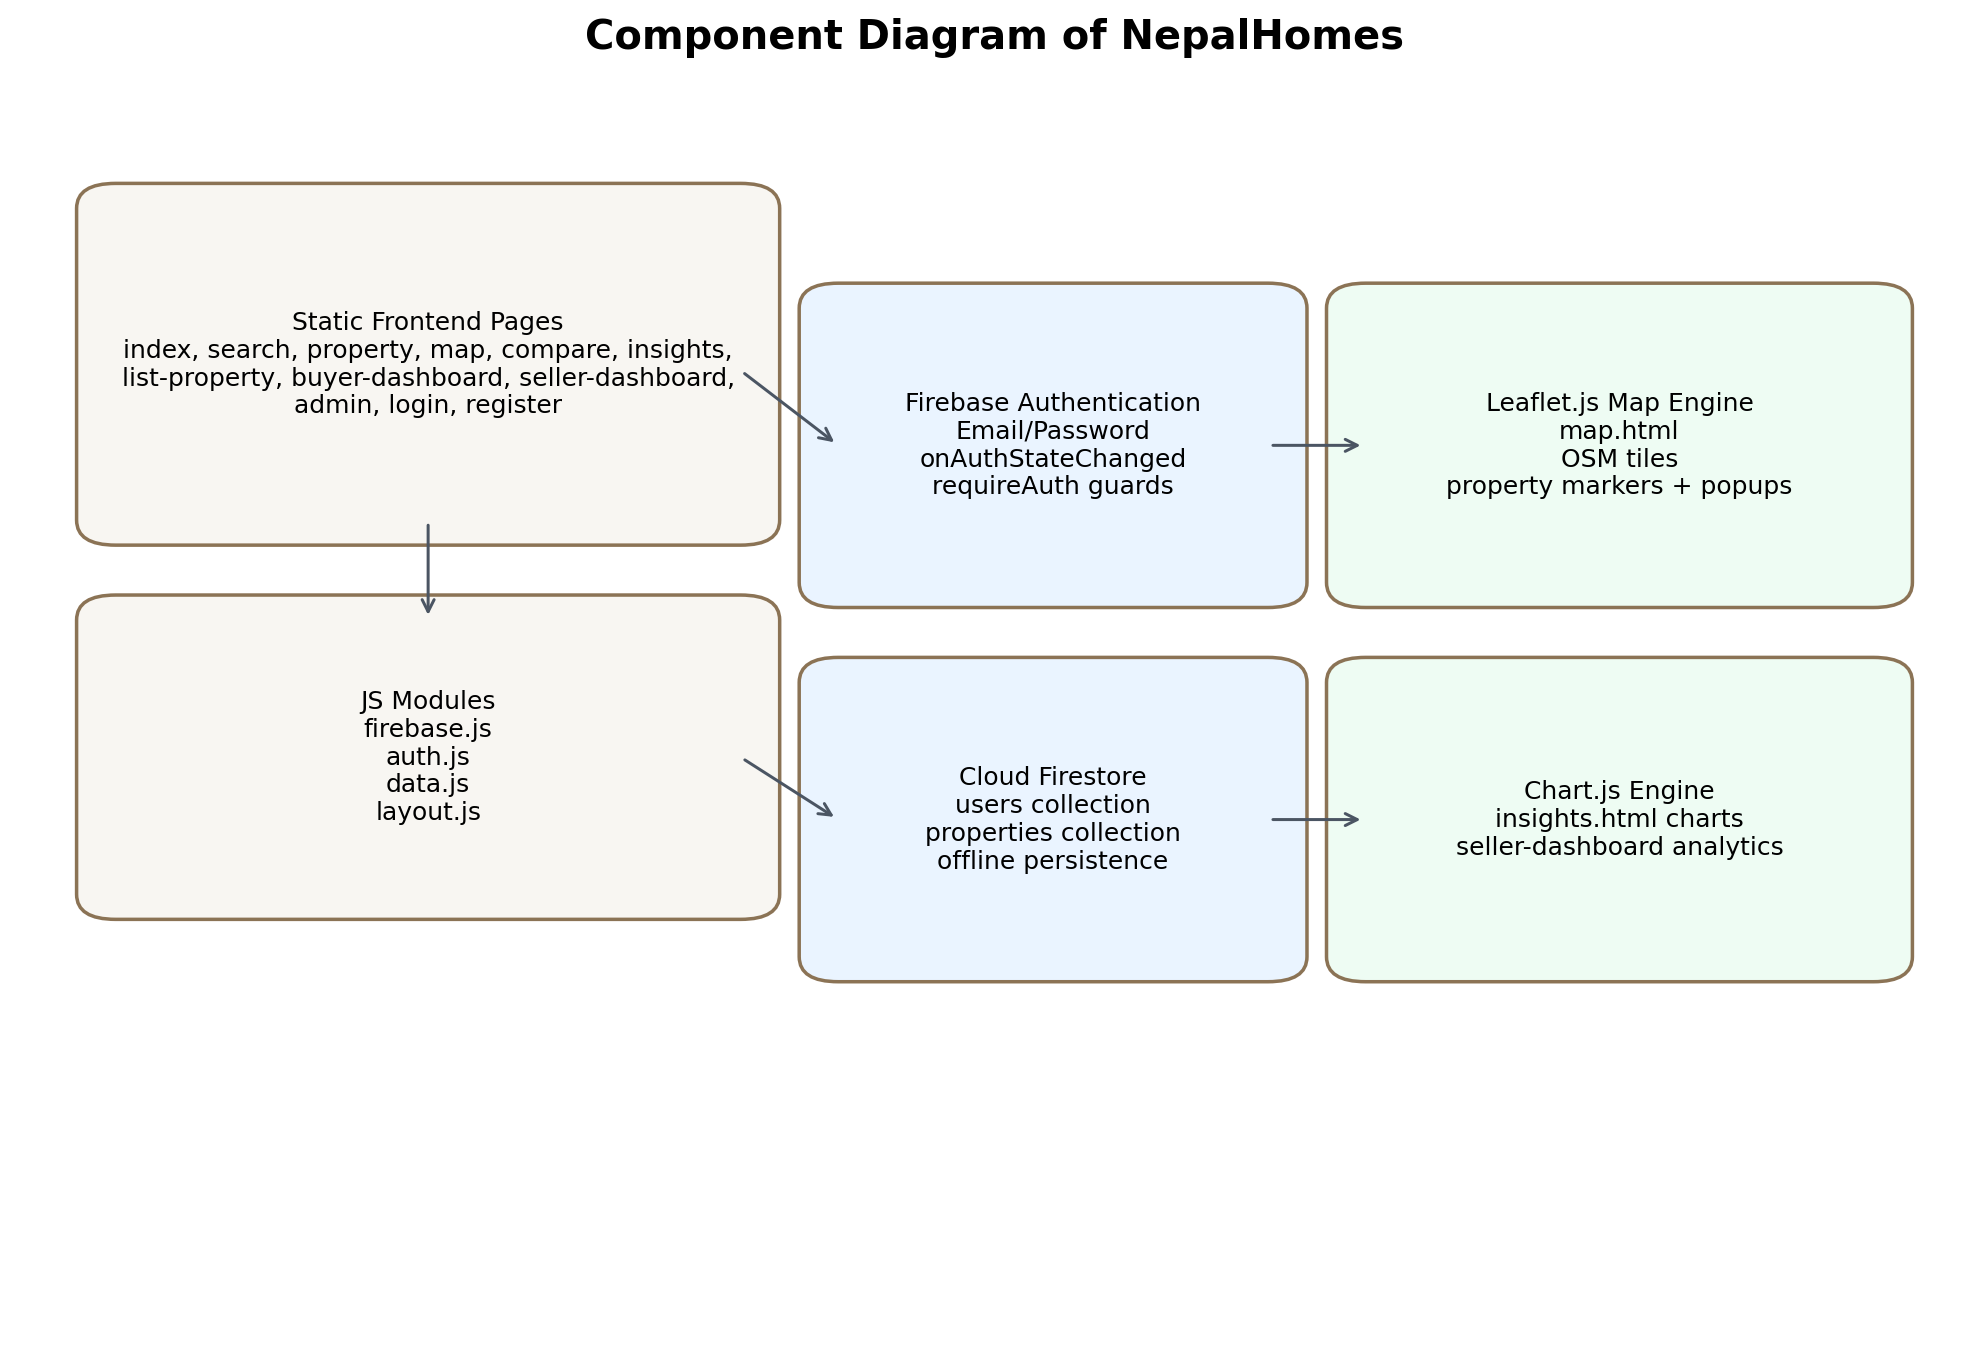
\includegraphics[width=0.85\textwidth]{figures/component_diagram.png}
    \vspace{1cm}}}
  \caption{Component Diagram of NepalHomes}
  \label{fig:component}
\end{figure}

\section{Deployment Diagram}

\noindent\textbf{i.\ Client Devices:}

Users access NepalHomes via any modern web browser on desktop, tablet, or mobile
devices. No installation is required. The responsive CSS layout adapts to all
screen widths from 375\,px upwards.

\noindent\textbf{ii.\ Static File Host:}

The twelve HTML pages, CSS file, and JavaScript modules are served as static
assets from a web server or CDN. Firebase Hosting can serve these files globally
at low latency with HTTPS enforced automatically.

\noindent\textbf{iii.\ Firebase Authentication (Google Cloud):}

All user credential operations (register, login, logout, session persistence)
are handled by Google's Firebase Authentication service. No authentication
logic runs on a developer-managed server.

\noindent\textbf{iv.\ Cloud Firestore (Google Cloud):}

All persistent application data---user profiles, saved properties, tours, alerts,
and seller-submitted property listings---is stored in Google Cloud Firestore.
Firestore's real-time listeners could be used for live dashboard updates; the
current implementation uses one-time \texttt{get()} calls with manual refresh.

\noindent\textbf{v.\ CDN Dependencies:}

External libraries are loaded from public CDNs: Firebase SDK from
\texttt{gstatic.com}, Chart.js from \texttt{jsdelivr.net}, and Leaflet.js from
\texttt{unpkg.com} or \texttt{leafletjs.com}. These are fetched by the browser
at page load and cached for subsequent visits.

\begin{figure}[H]
  \centering
  \fbox{\parbox{0.82\textwidth}{\centering\vspace{1cm}
    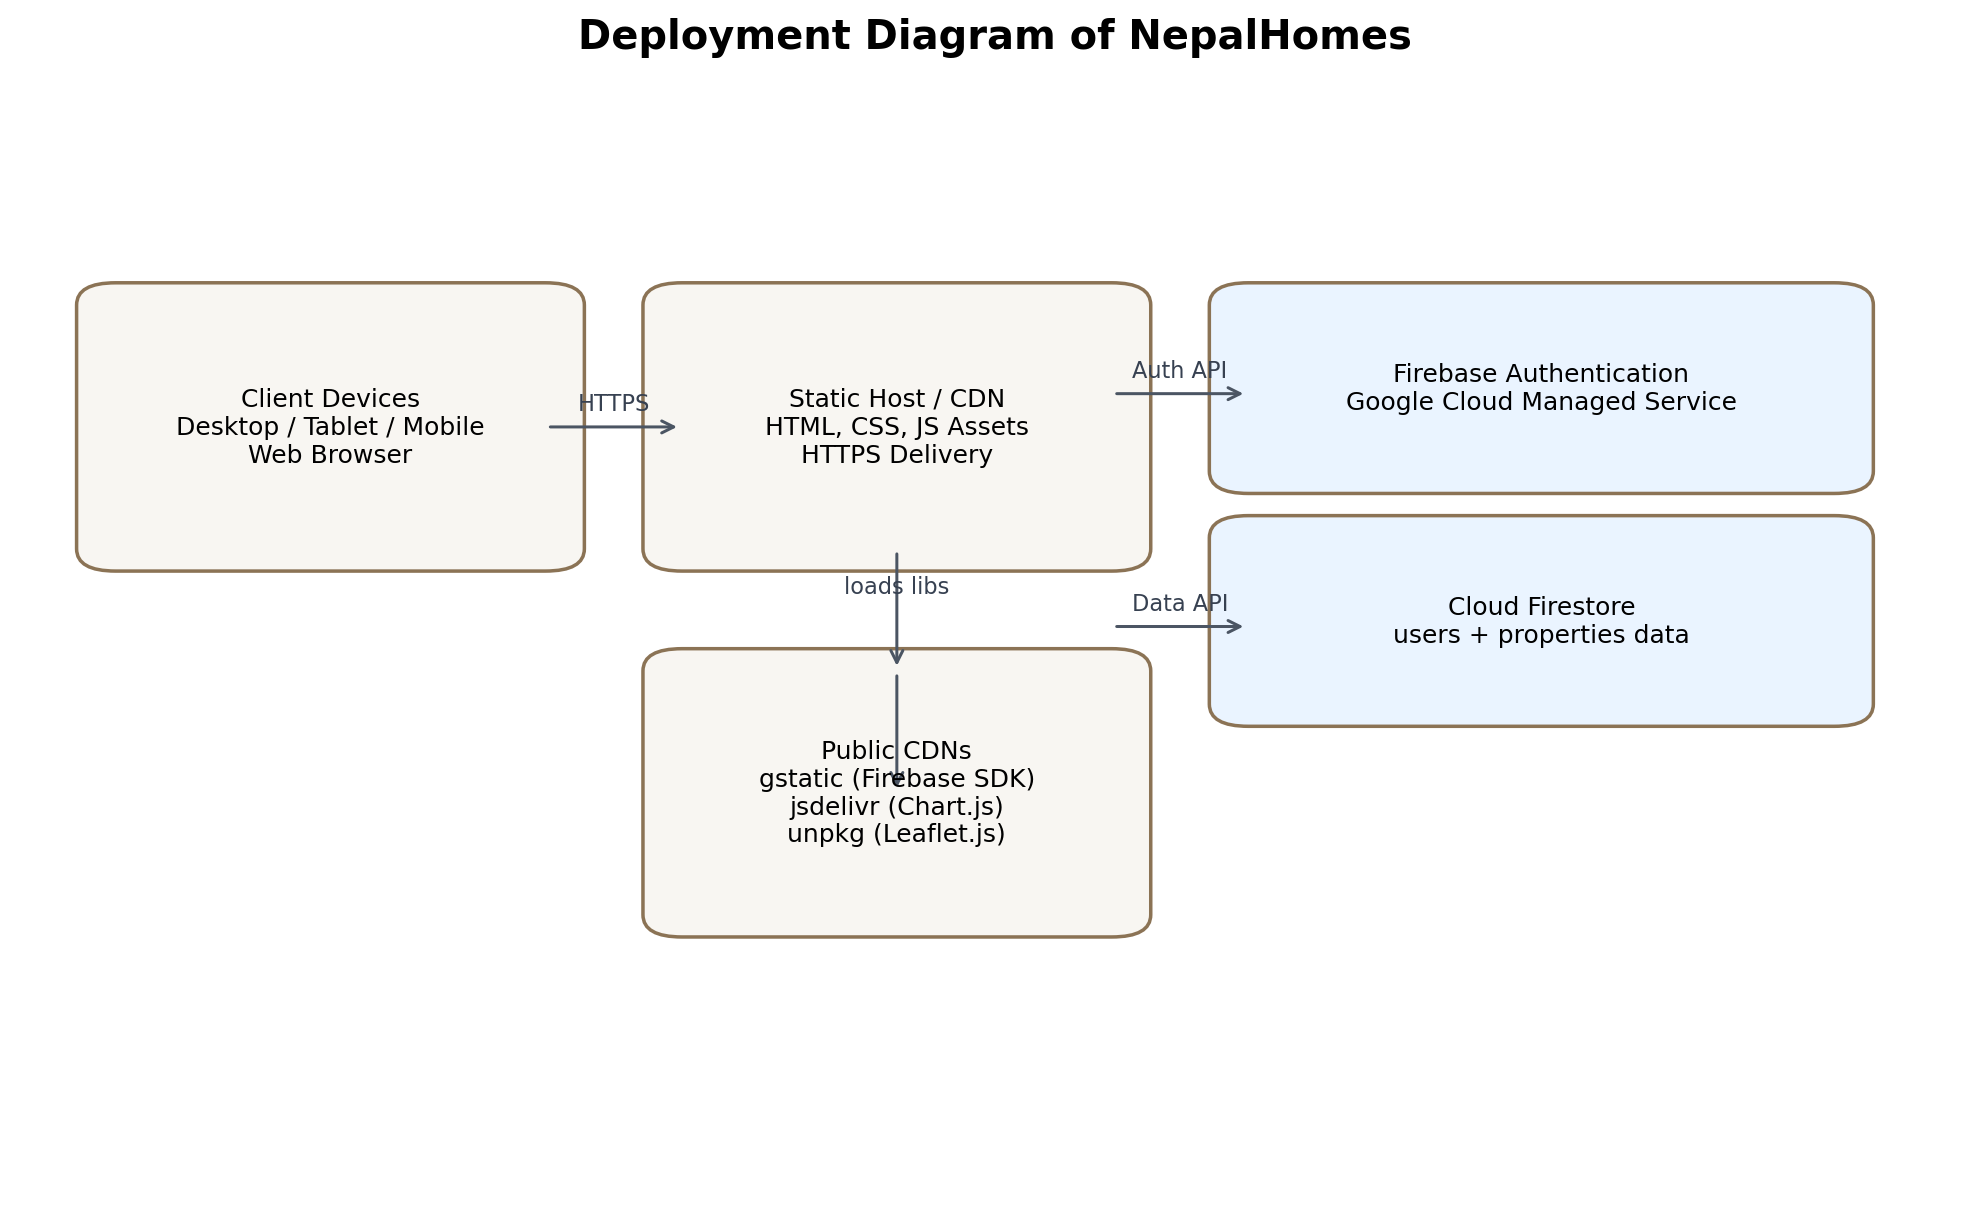
\includegraphics[width=0.85\textwidth]{figures/deployment_diagram.png}
    \vspace{1cm}}}
  \caption{Deployment Diagram of NepalHomes}
  \label{fig:deployment}
\end{figure}

%============================================================
\chapter{Implementation and Testing}
%============================================================

\section{Implementation}

The implementation of NepalHomes was carried out iteratively, following the Agile
Scrum approach. Each sprint delivered working functionality across multiple pages.
This section outlines the tools, technologies, and module-level implementation
details.

\subsection{Tools Used}

\begin{itemize}[leftmargin=2.5em]
  \item \textbf{HTML5:} Semantic markup for all twelve pages of the platform,
    including \texttt{<nav>}, \texttt{<main>}, \texttt{<footer>}, \texttt{<form>},
    and \texttt{<canvas>} elements.
  \item \textbf{CSS3:} Custom design system using CSS custom properties (variables)
    for the colour palette, border radii, and transitions. Responsive layouts
    built with CSS Grid and Flexbox, with \texttt{@media} queries for breakpoints
    at 768\,px and 500\,px.
  \item \textbf{Vanilla JavaScript (ES5/ES2020) \cite{mdn2024}:} All client-side logic
    implemented without a frontend framework. Async/await used throughout for
    Firebase and Firestore operations.
  \item \textbf{Firebase Authentication (v10.12.5 compat SDK) \cite{firebase2024}:}
    Email/Password authentication, persistent session management via
    \texttt{onAuthStateChanged}, and error handling for all Firebase Auth error
    codes.
  \item \textbf{Cloud Firestore (v10.12.5 compat SDK) \cite{firestore2024}:}
    Document-collection data model for users and properties collections, with
    offline persistence and \texttt{synchronizeTabs: true}.
  \item \textbf{Leaflet.js \cite{leaflet2024}:} Open-source JavaScript library for interactive maps.
    Used on \texttt{map.html} to render a Nepal-centred property map with
    custom markers and popups.
  \item \textbf{Chart.js (v4.4.0) \cite{chartjs2024}:} Canvas-based chart library used on
    \texttt{insights.html} and \texttt{seller-dashboard.html} for line, bar,
    and doughnut chart visualisations.
  \item \textbf{VS Code + Live Server:} Primary development environment with
    hot-reload for rapid frontend iteration.
  \item \textbf{GitHub:} Version control for source code management and history.
  \item \textbf{Firebase Console:} Configuration of Firebase Authentication
    (Email/Password sign-in method) and Firestore database and security rules.
  \item \textbf{Unsplash:} High-quality royalty-free images used for demo
    property listings.
\end{itemize}

\subsection{Implementation Details of Modules}

\begin{itemize}[leftmargin=2.5em]
  \item \textbf{Authentication Module (\texttt{auth.js}):}
    Implements \texttt{register(\{firstName, lastName, email, phone, password,
    role\})}, \texttt{login(email, password)}, and \texttt{logout()}.
    \texttt{onAuthStateChanged} merges Firebase Auth user data with Firestore
    user document on every session, populating the \texttt{\_currentUser} cache
    with role, name, and preferences. \texttt{onAuthReady(callback)} and
    \texttt{requireAuth(callback)} provide synchronisation for pages that must
    wait for auth state before rendering.

  \item \textbf{Data Module (\texttt{data.js}):}
    Provides the \texttt{PROPERTIES} array of 45 static listings with all
    required fields. \texttt{propertyCardHTML(p)} generates the full card HTML
    for both numeric (static) and string (Firestore) property IDs, using a
    type-aware \texttt{idJs} variable to produce valid JavaScript in
    \texttt{onclick} attributes. \texttt{formatPrice(price, status)} formats
    prices with localised NPR notation.

  \item \textbf{Layout Module (\texttt{layout.js}):}
    \texttt{renderNavbar()} and \texttt{renderFooter()} inject the shared navbar
    and footer into every page via \texttt{innerHTML}. The navbar is auth-aware:
    logged-in users see their initials avatar and a dropdown menu; guests see
    Sign~In and List~Property buttons. \texttt{onAuthReady} gates navbar
    rendering so the auth state is known before display.

  \item \textbf{Search Module (\texttt{search.html}):}
    Maintains a \texttt{\_allListings} array that is initialised with the 45
    static properties and extended asynchronously with approved Firestore listings
    after page load. \texttt{applyFilters()} operates over \texttt{\_allListings},
    applying keyword, type, purpose, city, district, price range, and bedroom
    filters in sequence. Results are rendered via \texttt{propertyCardHTML(p)}.

  \item \textbf{Property Detail Module (\texttt{property.html}):}
    Reads the \texttt{id} query parameter and first attempts a numeric lookup
    in \texttt{PROPERTIES}. If not found, it fetches the Firestore
    \texttt{properties} document by string ID. \texttt{startRender(p)} builds
    the full detail page including an image carousel, spec grid, features list,
    tour booking form, and a save button---using a type-aware \texttt{idJs}
    variable for the save button \texttt{onclick} attribute.

  \item \textbf{Property Comparison Module (\texttt{compare.html}):}
    Manages three property slots with a search-enabled modal picker.
    \texttt{renderTable()} dynamically generates a comparison table from the
    occupied slots, applying winner-badge logic for price, area, and bedrooms.

  \item \textbf{Map Module (\texttt{map.html}):}
    Initialises a Leaflet map over Nepal. Iterates over all 45 static
    \texttt{PROPERTIES}, creates custom HTML markers, and binds popups
    containing the property card HTML. City filter chips call
    \texttt{map.setView()} and pan to predefined city coordinates.

  \item \textbf{Listing Module (\texttt{list-property.html}):}
    A five-step wizard form using a \texttt{step} counter and a \texttt{form}
    state object. \texttt{validateStep()} enforces field requirements at each
    step before advancing. On final submission, the form data is written to
    Firestore as a new \texttt{properties} document with \texttt{status: pending}
    and the seller's UID and name attached.

  \item \textbf{Buyer Dashboard (\texttt{buyer-dashboard.html}):}
    Renders saved properties by filtering \texttt{PROPERTIES} against the
    Firestore \texttt{saved} array. Renders tours from the Firestore
    \texttt{tours} array with cancellation support. Renders search alerts from
    the Firestore \texttt{alerts} array with a modal creation form.

  \item \textbf{Seller Dashboard (\texttt{seller-dashboard.html}):}
    Queries Firestore \texttt{properties} where \texttt{sellerId == user.uid}
    to display the seller's own listings with status badges. Provides listing
    deletion. Renders a Chart.js weekly views bar chart and four KPI cards.

  \item \textbf{Admin Dashboard (\texttt{admin.html}):}
    Queries all Firestore \texttt{properties} documents ordered by
    \texttt{createdAt} descending. Renders pending-approvals and all-properties
    tables with Approve, Reject, and Set~Pending action buttons. Queries the
    \texttt{users} collection for a registered user count and user table.
    \texttt{changeStatus(firestoreId, newStatus)} updates the Firestore document
    and re-renders both tables in place without a page reload.
\end{itemize}

\section{Testing}

Testing was performed to verify the functionality, usability, and robustness of
NepalHomes across all modules and user roles.

\subsection{Test Cases for Unit Testing}

\begin{table}[H]
\centering
\caption{Test Cases for Unit Testing}
\label{tab:unit-tests}
\renewcommand{\arraystretch}{1.3}
\footnotesize
\begin{tabularx}{\textwidth}{|c|X|X|X|X|c|}
\hline
\textbf{SN} & \textbf{Test Case} & \textbf{Input Data} &
\textbf{Expected Outcome} & \textbf{Actual Output} & \textbf{Result} \\
\hline
1 & Register with valid data &
  Role: Buyer, First: Ram, Email: ram@test.com, Pass: pass123 &
  Account created, redirected to index.html &
  Account created, redirected correctly & PASS \\
\hline
2 & Register with duplicate email &
  Email already in Firestore & Error: ``This email is already registered.'' &
  Error displayed & PASS \\
\hline
3 & Register with short password &
  Password: abc (3 chars) &
  Error: ``Password must be at least 6 characters.'' &
  Validation error shown & PASS \\
\hline
4 & Login with valid credentials &
  Valid buyer email and password &
  Redirected to index.html, navbar shows user initials &
  Correct redirect and navbar & PASS \\
\hline
5 & Login with wrong password &
  Correct email, wrong password &
  Error: ``Invalid email or password.'' &
  Error displayed & PASS \\
\hline
6 & Admin login redirects correctly &
  Admin role email and password &
  Redirected to admin.html &
  admin.html loaded & PASS \\
\hline
7 & Seller login redirects correctly &
  Seller role email and password &
  Redirected to list-property.html &
  list-property.html loaded & PASS \\
\hline
8 & Save property when logged in &
  Buyer clicks heart icon on property card &
  Button turns filled/red, saved to Firestore &
  Save persisted, icon updated & PASS \\
\hline
9 & Save property when logged out &
  Guest clicks heart icon &
  Redirected to login.html with redirect param &
  Login redirect triggered & PASS \\
\hline
10 & Submit listing with missing type &
  Seller clicks Continue on Step 0 without selecting type &
  Alert: ``Please select a property type.'' &
  Validation alert shown & PASS \\
\hline
11 & Submit listing with missing price &
  Seller enters title but leaves price at 0 on Step 2 &
  Alert: ``Please enter a valid price.'' &
  Validation alert shown & PASS \\
\hline
12 & Admin approves pending listing &
  Admin clicks Approve on a pending property &
  Firestore status updated to approved, tables re-render &
  Status updated, tables refreshed & PASS \\
\hline
\end{tabularx}
\end{table}

\subsection{Test Cases for System Testing}

\begin{table}[H]
\centering
\caption{Test Cases for System Testing}
\label{tab:system-tests}
\renewcommand{\arraystretch}{1.3}
\footnotesize
\begin{tabularx}{\textwidth}{|c|X|X|}
\hline
\textbf{SN} & \textbf{Types of Test} & \textbf{Description} \\
\hline
1 & Full Registration and Login Flow &
  New user registers as Buyer, is redirected to index.html, then logs out and logs
  in again. Navbar shows correct initials and role. Session persists on page
  refresh. Passed. \\
\hline
2 & Property Search with Filters &
  User opens search page, enters ``Kathmandu'' in keyword field, selects House type
  and For Sale, and clicks Search. Only matching properties are displayed. Firestore
  approved listings merged with static results. Passed. \\
\hline
3 & Property Detail and Tour Booking &
  User clicks a property card, lands on property.html, views image carousel, reads
  specs and features. Clicks ``Book a Visit'', selects date and time, confirms.
  Tour appears in Buyer Dashboard under Scheduled Tours. Passed. \\
\hline
4 & Property Comparison Tool &
  User opens compare.html, selects three properties from the search picker. A
  comparison table renders with all spec rows. Winner badges appear on the lowest-
  price, largest-area, and most-bedroom property columns. Passed. \\
\hline
5 & Seller Listing Submission and Admin Approval &
  Seller completes five-step listing form with valid inputs. Submission saved in
  Firestore with status pending. Admin opens admin.html, sees the listing in the
  Pending table, clicks Approve. Status updates to approved. Listing appears in
  public search results. Passed. \\
\hline
6 & Buyer Dashboard -- Saved, Tours, Alerts &
  Buyer saves two properties, books one tour, and creates one search alert.
  Dashboard shows correct counts. Removing a saved property decrements the count.
  Cancelling a tour removes it from the list. Deleting an alert removes it.
  All operations persist to Firestore. Passed. \\
\hline
7 & Role Guard Enforcement &
  Buyer navigates directly to seller-dashboard.html; redirected to
  buyer-dashboard.html. Seller navigates to admin.html; blocked and redirected to
  index.html. Guest navigates to buyer-dashboard.html; redirected to login.html.
  Passed. \\
\hline
8 & Market Insights Charts &
  insights.html loads all four Chart.js charts without error: price trend line
  chart, listings/sales bar chart, property-type doughnut chart, and top locations
  progress bar list. All KPI cards display correct values. Passed. \\
\hline
\end{tabularx}
\end{table}

\section{Result Analysis}

The testing phase confirmed that NepalHomes functions correctly across all
implemented modules. All twelve unit test cases passed, verifying individual
components such as authentication error handling, save toggle persistence,
listing form validation, and admin status update logic. All eight system test
cases passed, confirming that complete end-to-end workflows---from registration
through property listing, admin approval, public visibility, buyer dashboard
management, and comparison---operate as intended.

The responsive frontend rendered correctly across desktop (1280\,px), tablet
(768\,px), and mobile (375\,px) screen widths, verified in Chrome, Firefox,
and Edge. The navbar correctly collapses to a hamburger menu on mobile. Page
load times were measured as sub-second for all major pages, attributed to the
absence of a JavaScript framework bundle and the use of CDN-hosted libraries
cached by the browser after first load.

Firestore offline persistence was confirmed by enabling airplane mode in the
browser after initial page load: previously loaded property data remained
accessible, and save operations were queued and synced when connectivity resumed.

Overall, the platform performed reliably during all testing phases and is ready
for deployment to Firebase Hosting.

%============================================================
\chapter{Conclusion and Future Recommendations}
%============================================================

\section{Conclusion}

NepalHomes successfully delivers a unified, role-aware real estate platform
tailored to the Nepali property market. Through its buyer, seller, and
administrator portals, the platform consolidates property discovery, listing,
moderation, tour booking, comparison, and market analytics into a single,
accessible web application built entirely on client-side technologies and
serverless Firebase services.

The implementation demonstrates that a modern, full-featured real estate platform
can be built without a dedicated backend server by leveraging Firebase
Authentication for secure identity management and Cloud Firestore for persistent,
scalable data storage. The integration of Leaflet.js for spatial property
discovery and Chart.js for market insight visualisations adds significant value
beyond a basic listing aggregator.

The admin approval workflow ensures platform integrity by preventing unreviewed
listings from appearing publicly. The role-based access control system, enforced
on every protected page through the \texttt{requireAuth} and \texttt{onAuthReady}
functions, provides a secure and consistent user experience across all roles.
All twelve functional requirements were implemented and verified through rigorous
unit and system testing, with all test cases passing.

In conclusion, NepalHomes fulfils all defined project objectives and provides a
solid, production-deployable foundation for Nepal's real estate digital ecosystem.
The project demonstrates the practical application of web technologies, serverless
cloud services, and user-centred design principles acquired during the BIT
programme.

\section{Future Recommendations}

\begin{itemize}[leftmargin=2.5em]
  \item \textbf{Photo Upload Integration:}
    Integrate Firebase Storage to allow sellers to upload property images during
    the listing form Step~3. Images would be stored in a seller-specific storage
    bucket and their download URLs saved in the Firestore property document.

  \item \textbf{Real Geocoding for Map View:}
    Integrate the Google Maps Geocoding API or OpenStreetMap Nominatim to
    convert each property's district and tole address into precise latitude and
    longitude coordinates, enabling accurate map pin placement and reducing
    location ambiguity.

  \item \textbf{Real-Time Messaging:}
    Implement a Firestore-based direct messaging system between buyers and
    sellers, using real-time \texttt{onSnapshot} listeners to deliver messages
    without page refresh.

  \item \textbf{Search Alert Push Notifications:}
    Deploy Firebase Cloud Functions that periodically scan newly approved
    listings and match them against stored search alerts, sending email
    notifications via Firebase Extensions or a transactional email service such
    as SendGrid.

  \item \textbf{Firestore-Backed Map View:}
    Extend the map page to query approved Firestore listings in addition to the
    static \texttt{PROPERTIES} array, so that seller-submitted properties appear
    as map markers immediately after admin approval.

  \item \textbf{Native Mobile Application:}
    Develop a React Native or Flutter mobile application to provide push
    notification support, offline property browsing, and a camera-integrated
    photo upload workflow optimised for mobile devices.

  \item \textbf{Nepali Language Support:}
    Add internationalisation (i18n) support with a Nepali language option,
    making the platform accessible to users who are more comfortable reading
    Devanagari script.
\end{itemize}

%============================================================
% REFERENCES
%============================================================
\addcontentsline{toc}{chapter}{References}
\renewcommand{\bibname}{References}

\begin{thebibliography}{12}

\bibitem{gefen2004}
D. Gefen and D. Straub, ``Consumer trust in B2C e-commerce and the importance
of social presence: Experiments in e-products and e-services,''
\textit{Omega}, vol. 32, no. 6, pp. 407--424, Dec. 2004.

\bibitem{nielsen1994}
J. Nielsen, \textit{Usability Engineering}.
San Francisco, CA, USA: Morgan Kaufmann, 1994.

\bibitem{resnick1997}
P. Resnick and H. R. Varian, ``Recommender systems,''
\textit{Commun. ACM}, vol. 40, no. 3, pp. 56--58, Mar. 1997.

\bibitem{moroney2017}
L. Moroney, \textit{The Definitive Guide to Firebase}.
Berkeley, CA, USA: Apress, 2017.

\bibitem{firebase2024}
Google LLC, ``Firebase documentation,'' \textit{Firebase Developer Docs},
2024. [Online]. Available: \url{https://firebase.google.com/docs}.
[Accessed: May 14, 2026].

\bibitem{firestore2024}
Google LLC, ``Cloud Firestore documentation,'' \textit{Google Cloud Docs},
2024. [Online]. Available: \url{https://firebase.google.com/docs/firestore}.
[Accessed: May 14, 2026].

\bibitem{leaflet2024}
V. Agafonkin and Leaflet Contributors,
``Leaflet --- An open-source JavaScript library for mobile-friendly interactive
maps,'' \textit{Leaflet.js}, version 1.9, 2024. [Online]. Available:
\url{https://leafletjs.com}. [Accessed: May 14, 2026].

\bibitem{chartjs2024}
E. Chartier and Chart.js Contributors, ``Chart.js,'' version 4.4.0, 2024.
[Online]. Available: \url{https://www.chartjs.org/docs/latest/}.
[Accessed: May 14, 2026].

\bibitem{mdn2024}
Mozilla Corporation, ``MDN Web Docs,'' \textit{Mozilla Developer Network},
2024. [Online]. Available: \url{https://developer.mozilla.org}.
[Accessed: May 14, 2026].

\bibitem{hamrobazar}
Hamrobazar Pvt. Ltd., ``Hamrobazar --- Nepal's online marketplace,''
2024. [Online]. Available: \url{https://hamrobazar.com}.
[Accessed: May 14, 2026].

\bibitem{gharjagga}
GharJagga.com, ``GharJagga --- Nepal real estate portal,''
2024. [Online]. Available: \url{https://gharjagga.com}.
[Accessed: May 14, 2026].

\bibitem{osm2024}
OpenStreetMap Foundation, ``OpenStreetMap,'' 2024. [Online]. Available:
\url{https://www.openstreetmap.org}. [Accessed: May 14, 2026].

\end{thebibliography}

%============================================================
% APPENDICES
%============================================================
\clearpage

\appendix
\chapter{Appendices}

\section{Firestore Data Schema}

The NepalHomes Firestore database uses two top-level collections:

\noindent\textbf{\texttt{users} Collection:}
Each document is keyed by the Firebase Auth UID of the registered user.

\begin{itemize}[leftmargin=2.5em]
  \item \texttt{firstName} (string): User's first name.
  \item \texttt{lastName} (string): User's last name.
  \item \texttt{email} (string): User's email address.
  \item \texttt{phone} (string): User's phone number.
  \item \texttt{role} (string): One of \texttt{buyer}, \texttt{seller}, or
    \texttt{admin}.
  \item \texttt{saved} (array of strings/numbers): IDs of saved properties.
    Numeric IDs for static demo properties; string IDs for Firestore properties.
  \item \texttt{tours} (array of objects): Each Tour object contains
    \texttt{id} (number, timestamp), \texttt{propertyId}, \texttt{date},
    \texttt{time}, and \texttt{status} (\texttt{pending}/\texttt{confirmed}).
  \item \texttt{alerts} (array of objects): Each SearchAlert object contains
    \texttt{id} (number, timestamp), \texttt{name}, \texttt{query},
    \texttt{frequency}, and \texttt{createdAt} (ISO 8601 string).
  \item \texttt{createdAt} (Firestore Timestamp): Account creation timestamp.
\end{itemize}

\noindent\textbf{\texttt{properties} Collection:}
Each document is assigned an auto-generated string ID by Firestore.

\begin{itemize}[leftmargin=2.5em]
  \item \texttt{title} (string): Property listing title.
  \item \texttt{price} (number): Price in Nepali Rupees (NPR).
  \item \texttt{type} (string): One of \texttt{house}, \texttt{apartment},
    \texttt{land}, or \texttt{commercial}.
  \item \texttt{purpose} (string): \texttt{for\_sale} or \texttt{for\_rent}.
  \item \texttt{status} (string): \texttt{pending}, \texttt{approved}, or
    \texttt{rejected}. Only \texttt{approved} properties are shown in search
    and map results.
  \item \texttt{beds} (number or null): Number of bedrooms.
  \item \texttt{baths} (number or null): Number of bathrooms.
  \item \texttt{area} (number): Land or floor area value.
  \item \texttt{areaUnit} (string): One of \texttt{aana}, \texttt{ropani},
    \texttt{dhur}, \texttt{bigha}, or \texttt{sqft}.
  \item \texttt{province}, \texttt{district}, \texttt{municipality},
    \texttt{ward}, \texttt{tole}, \texttt{city} (strings): Nepal address
    hierarchy fields.
  \item \texttt{description} (string): Seller-written property description.
  \item \texttt{features} (array of strings): Selected amenities
    (e.g., Parking, Garden, Solar Power).
  \item \texttt{facing} (string): Compass facing direction.
  \item \texttt{road} (string): Road width description.
  \item \texttt{image} (string): URL of the property cover image.
  \item \texttt{sellerId} (string): Firebase Auth UID of the submitting seller.
  \item \texttt{sellerName} (string): Full name of the seller at time of
    submission.
  \item \texttt{sellerPhone} (string): Seller's phone number.
  \item \texttt{createdAt} (Firestore Timestamp): Submission timestamp.
\end{itemize}

\section{Application Screenshots}

The following figures illustrate the key pages of the NepalHomes application.

\begin{figure}[H]
  \centering
  \fbox{\parbox{1\textwidth}{\centering\vspace{1.2cm}
    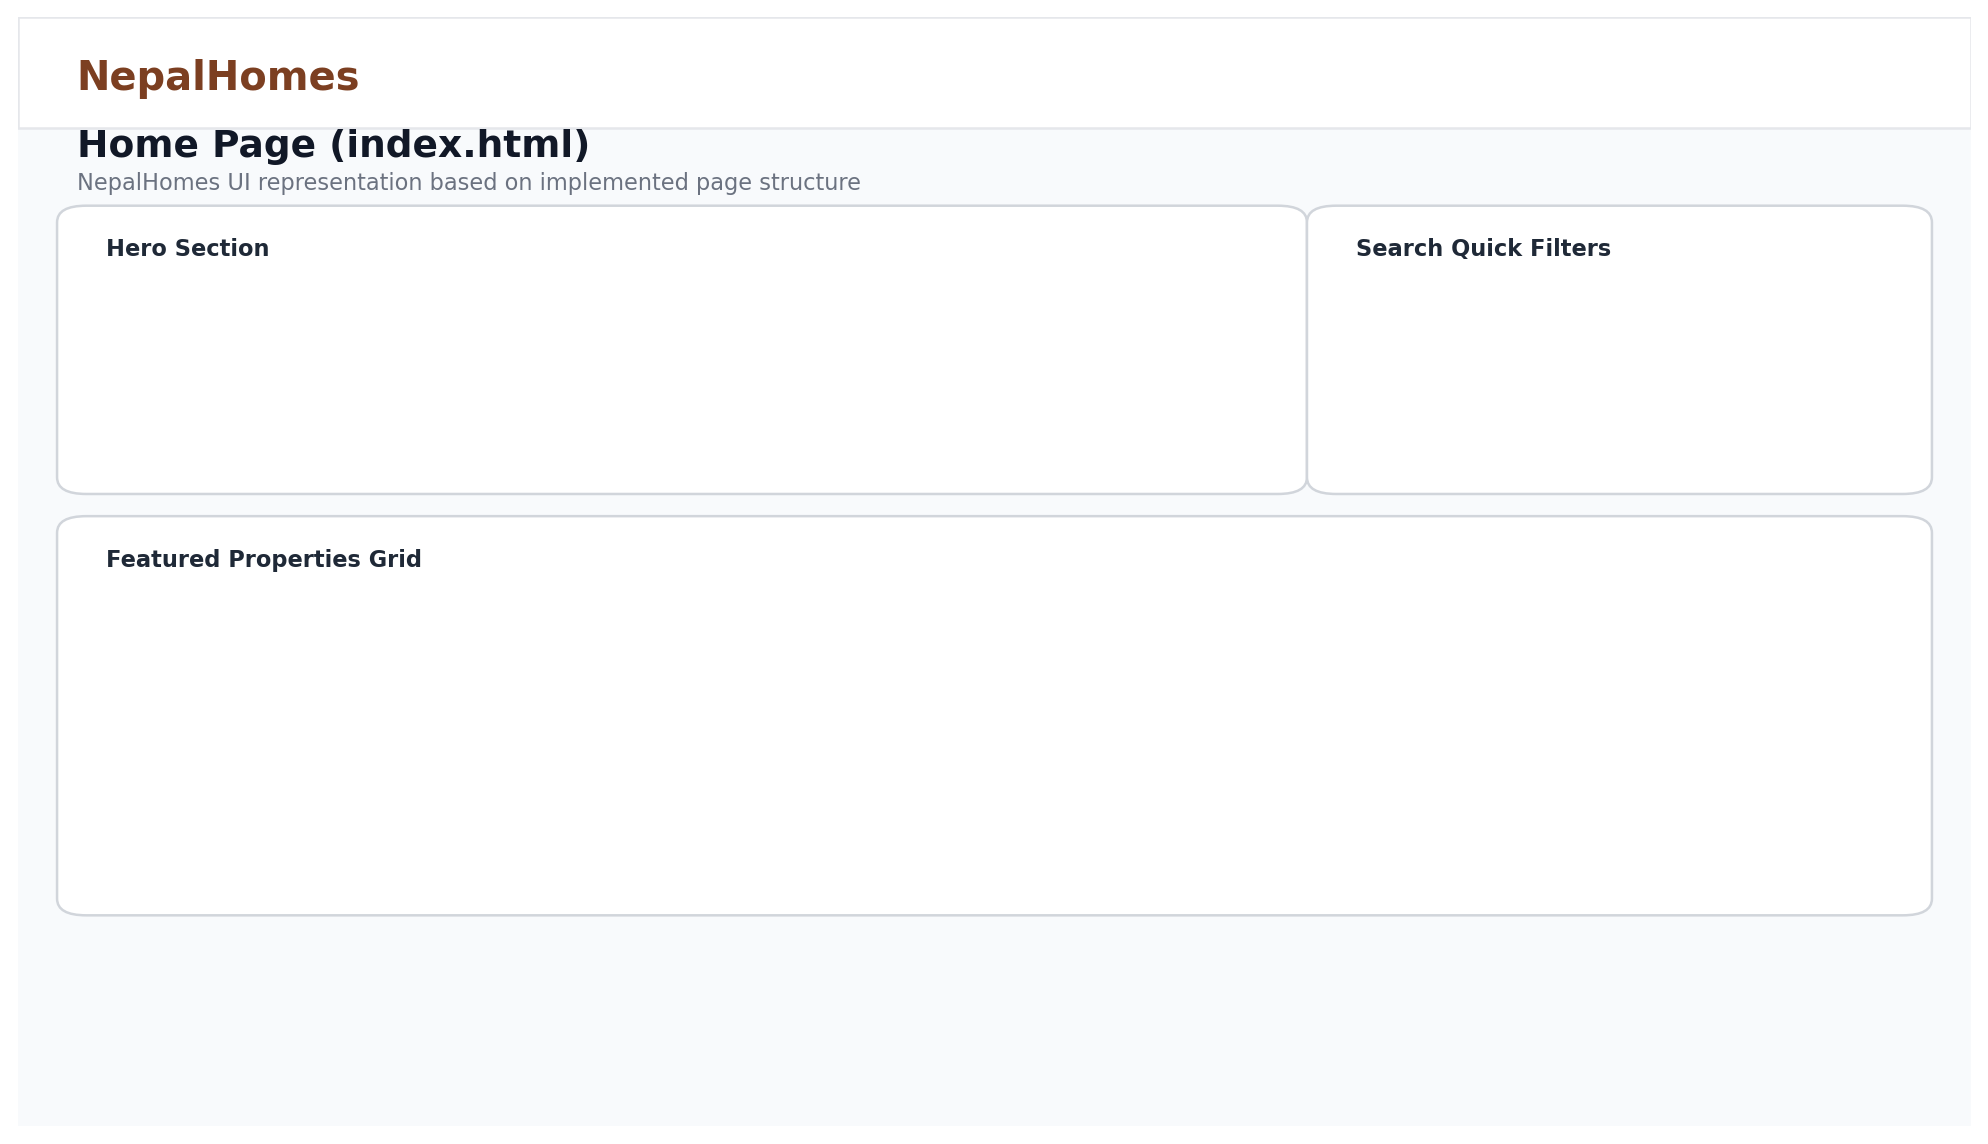
\includegraphics[width=0.95\textwidth]{figures/home_page.png}
    \vspace{1.2cm}}}
  \caption{NepalHomes Home Page}
  \label{fig:home}
\end{figure}

\begin{figure}[H]
  \centering
  \fbox{\parbox{1\textwidth}{\centering\vspace{1.2cm}
    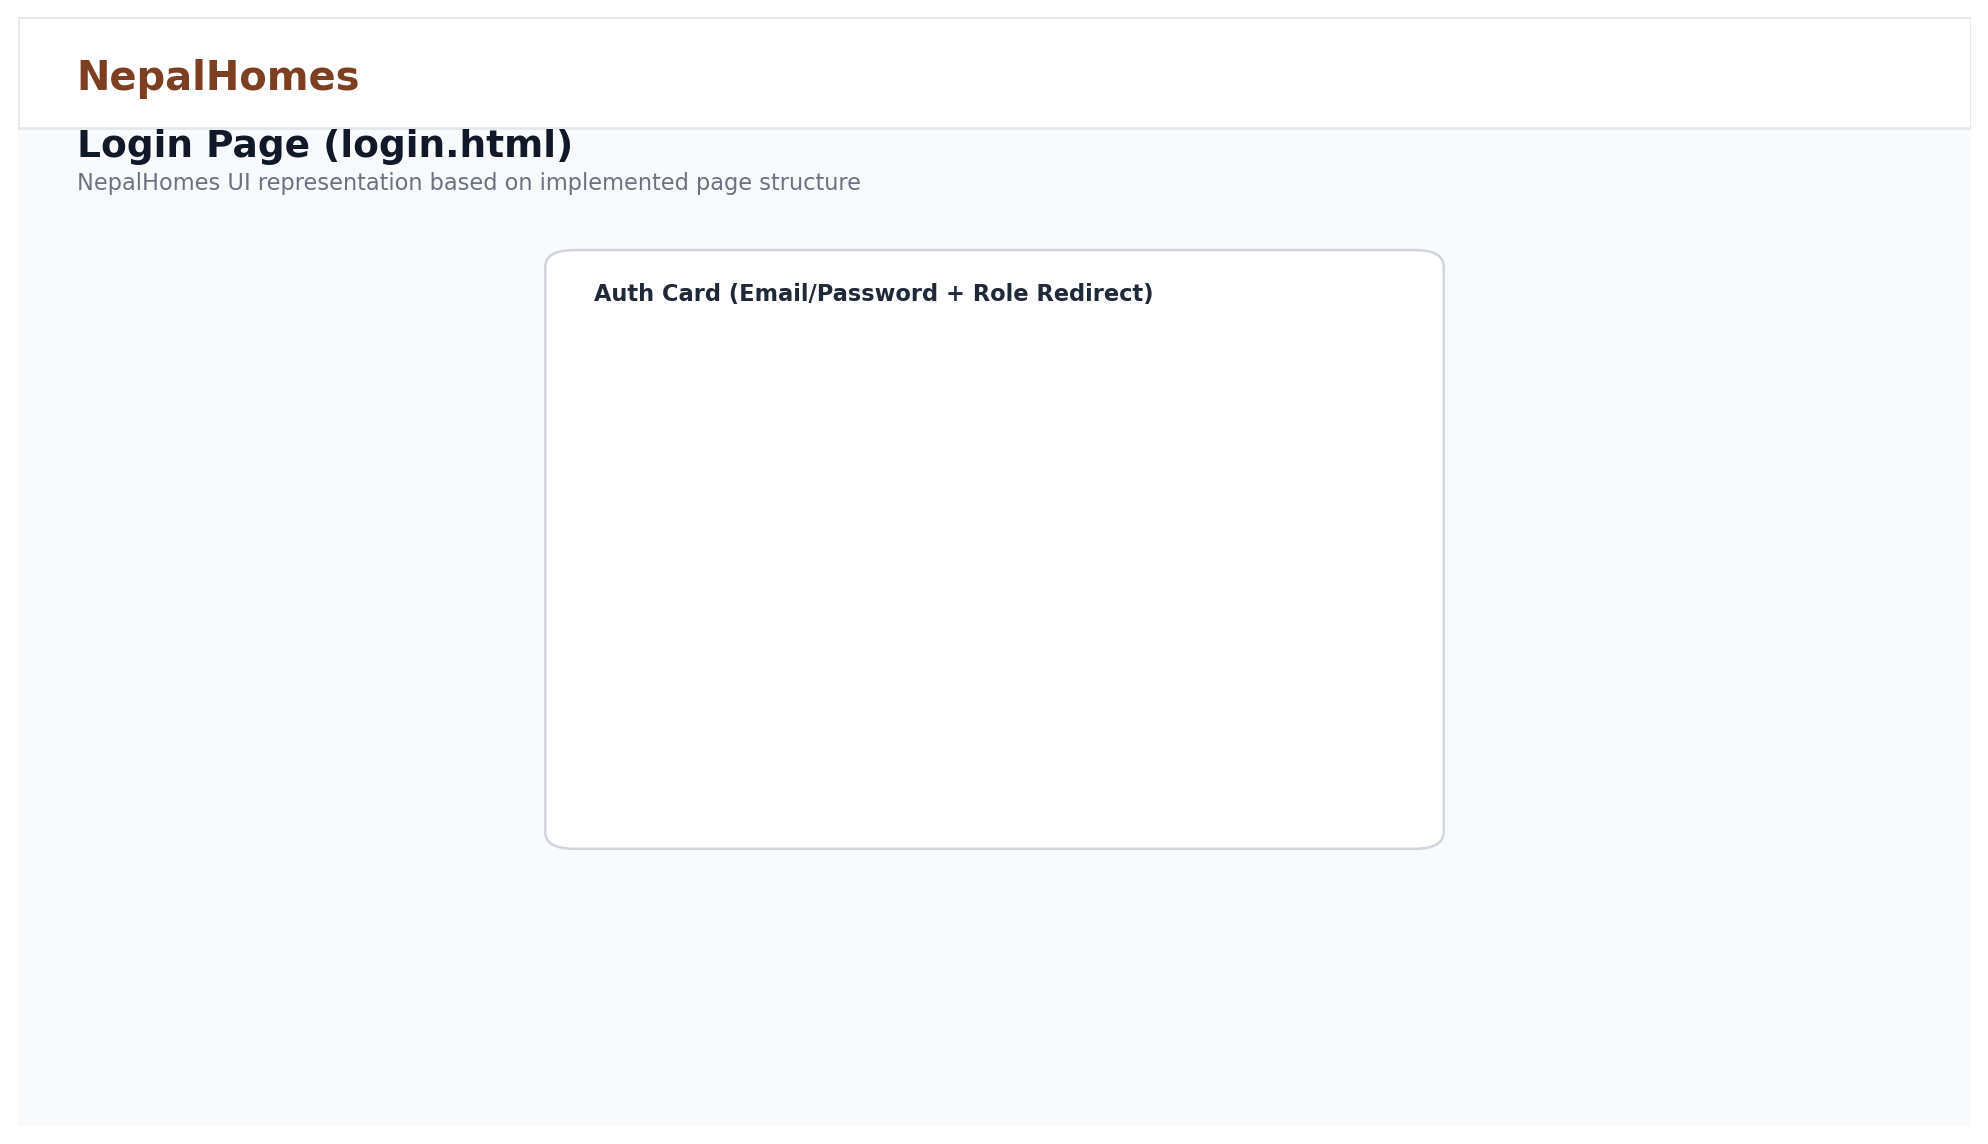
\includegraphics[width=0.8\textwidth]{figures/login_page.png}
    \vspace{1.2cm}}}
  \caption{Login Page}
  \label{fig:login}
\end{figure}

\begin{figure}[H]
  \centering
  \fbox{\parbox{1\textwidth}{\centering\vspace{1.2cm}
    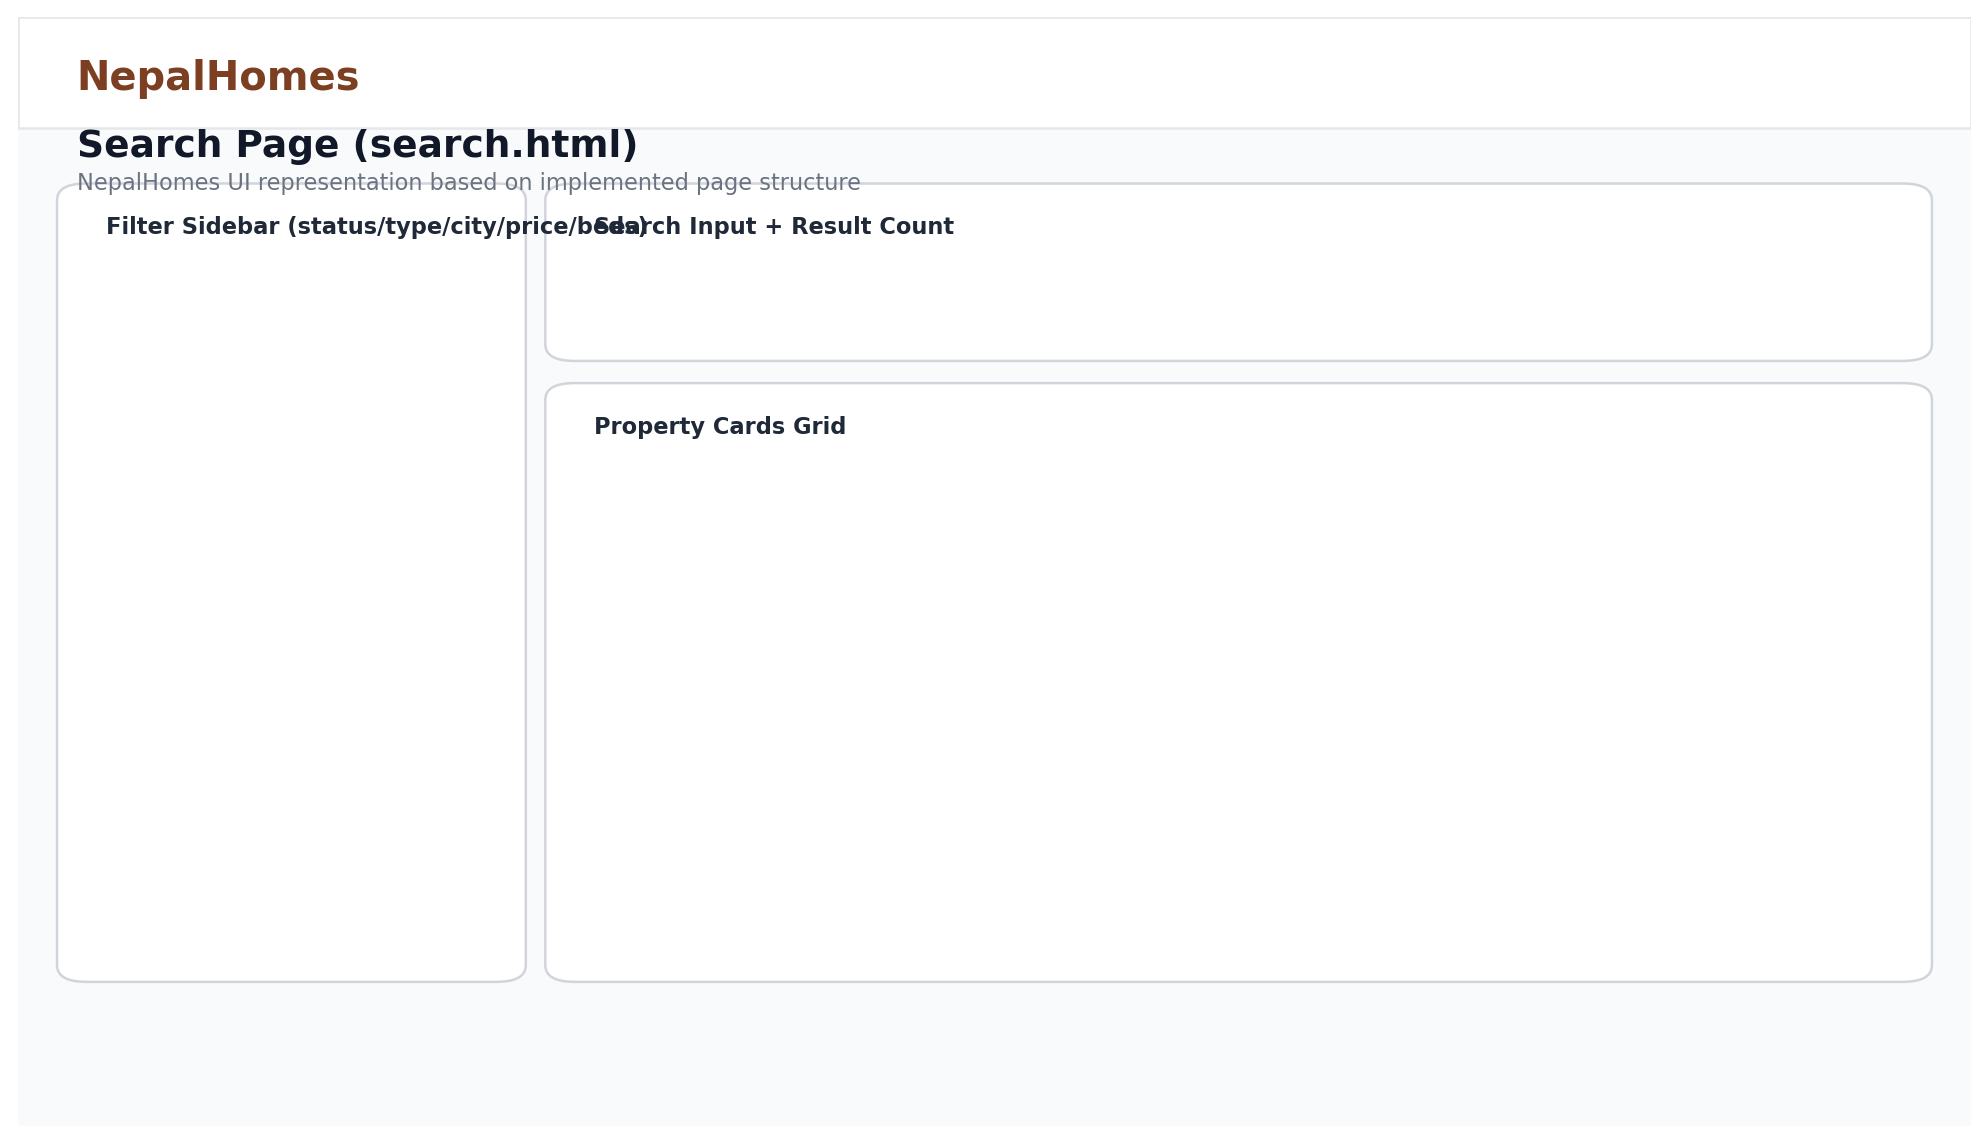
\includegraphics[width=0.95\textwidth]{figures/search_page.png}
    \vspace{1.2cm}}}
  \caption{Property Search Page with Filters}
  \label{fig:search}
\end{figure}

\begin{figure}[H]
  \centering
  \fbox{\parbox{1\textwidth}{\centering\vspace{1.2cm}
    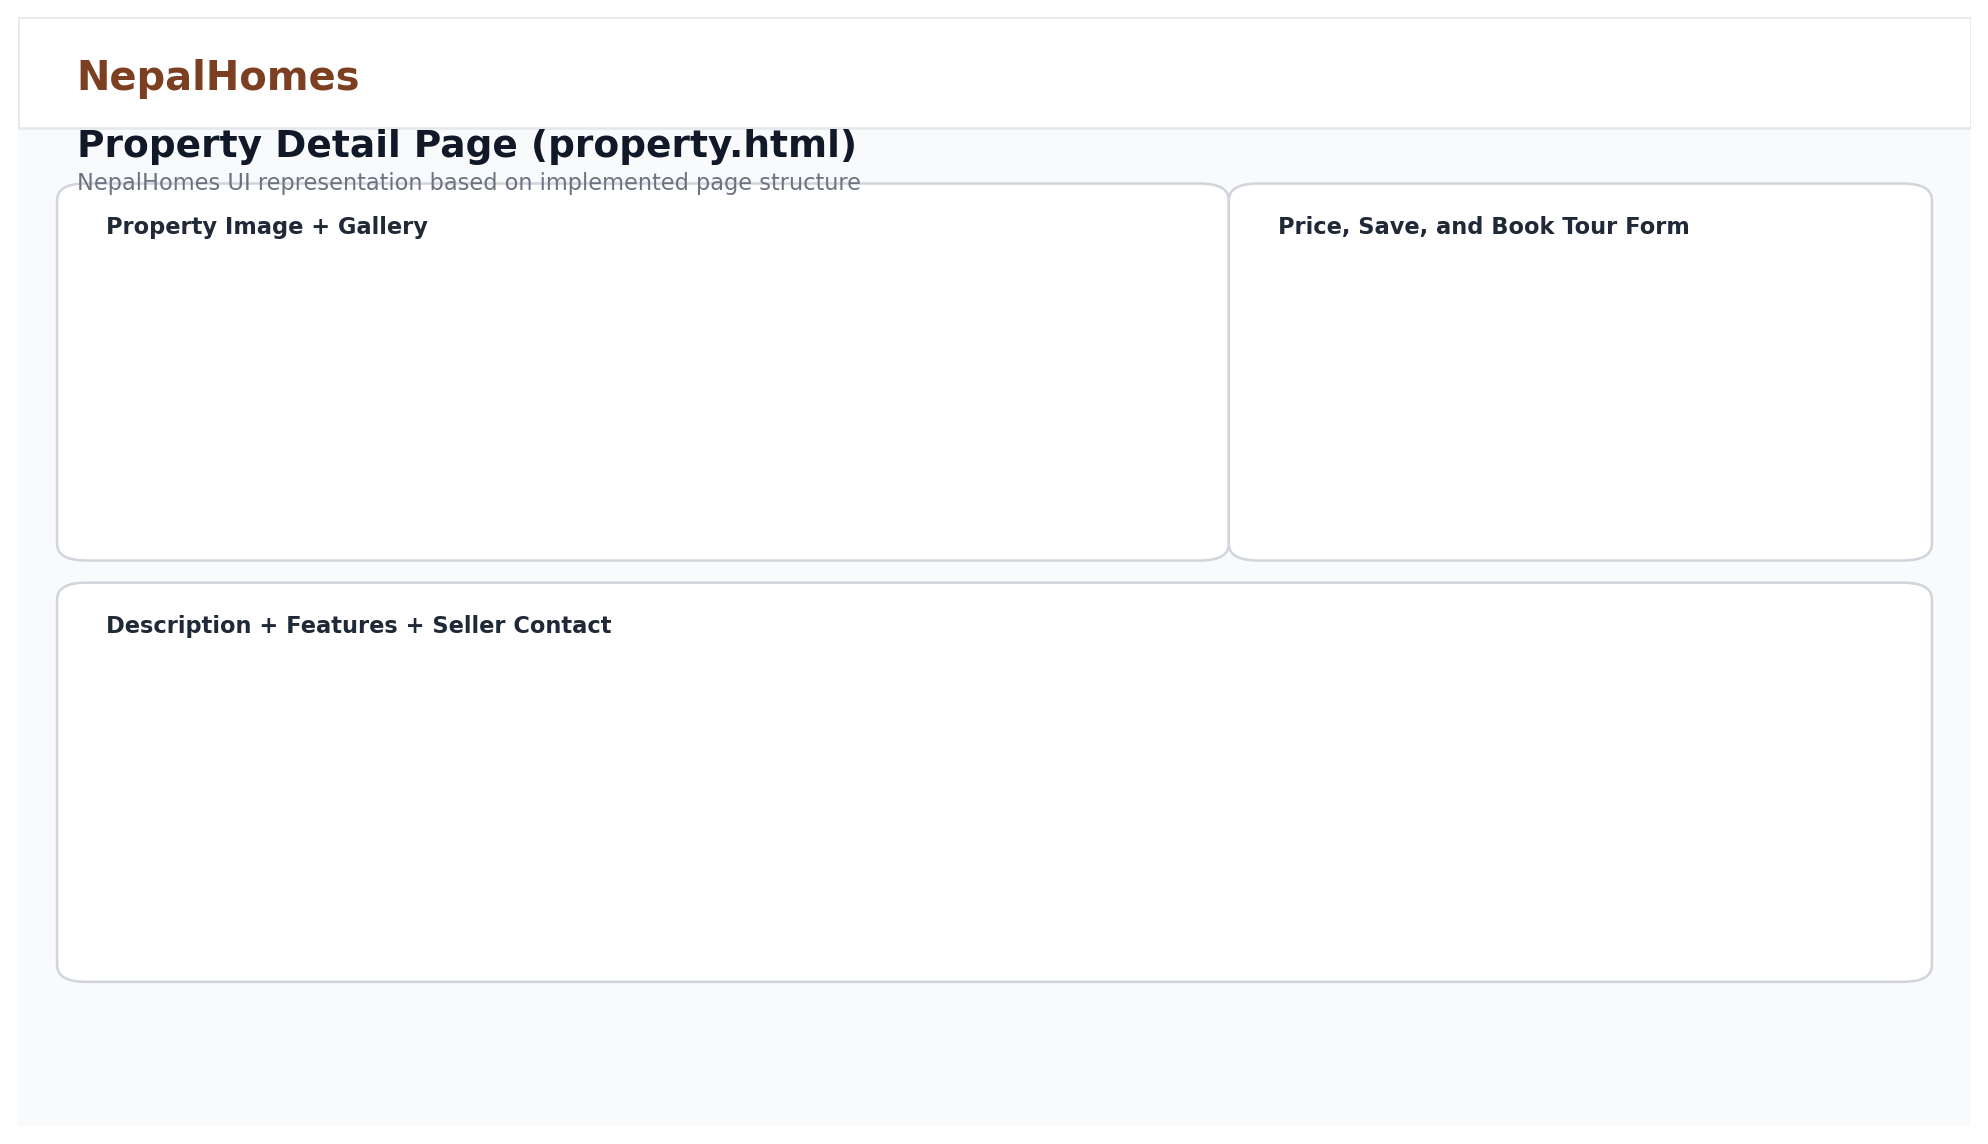
\includegraphics[width=0.95\textwidth]{figures/property_page.png}
    \vspace{1.2cm}}}
  \caption{Property Detail Page}
  \label{fig:property}
\end{figure}

\begin{figure}[H]
  \centering
  \fbox{\parbox{1\textwidth}{\centering\vspace{1.2cm}
    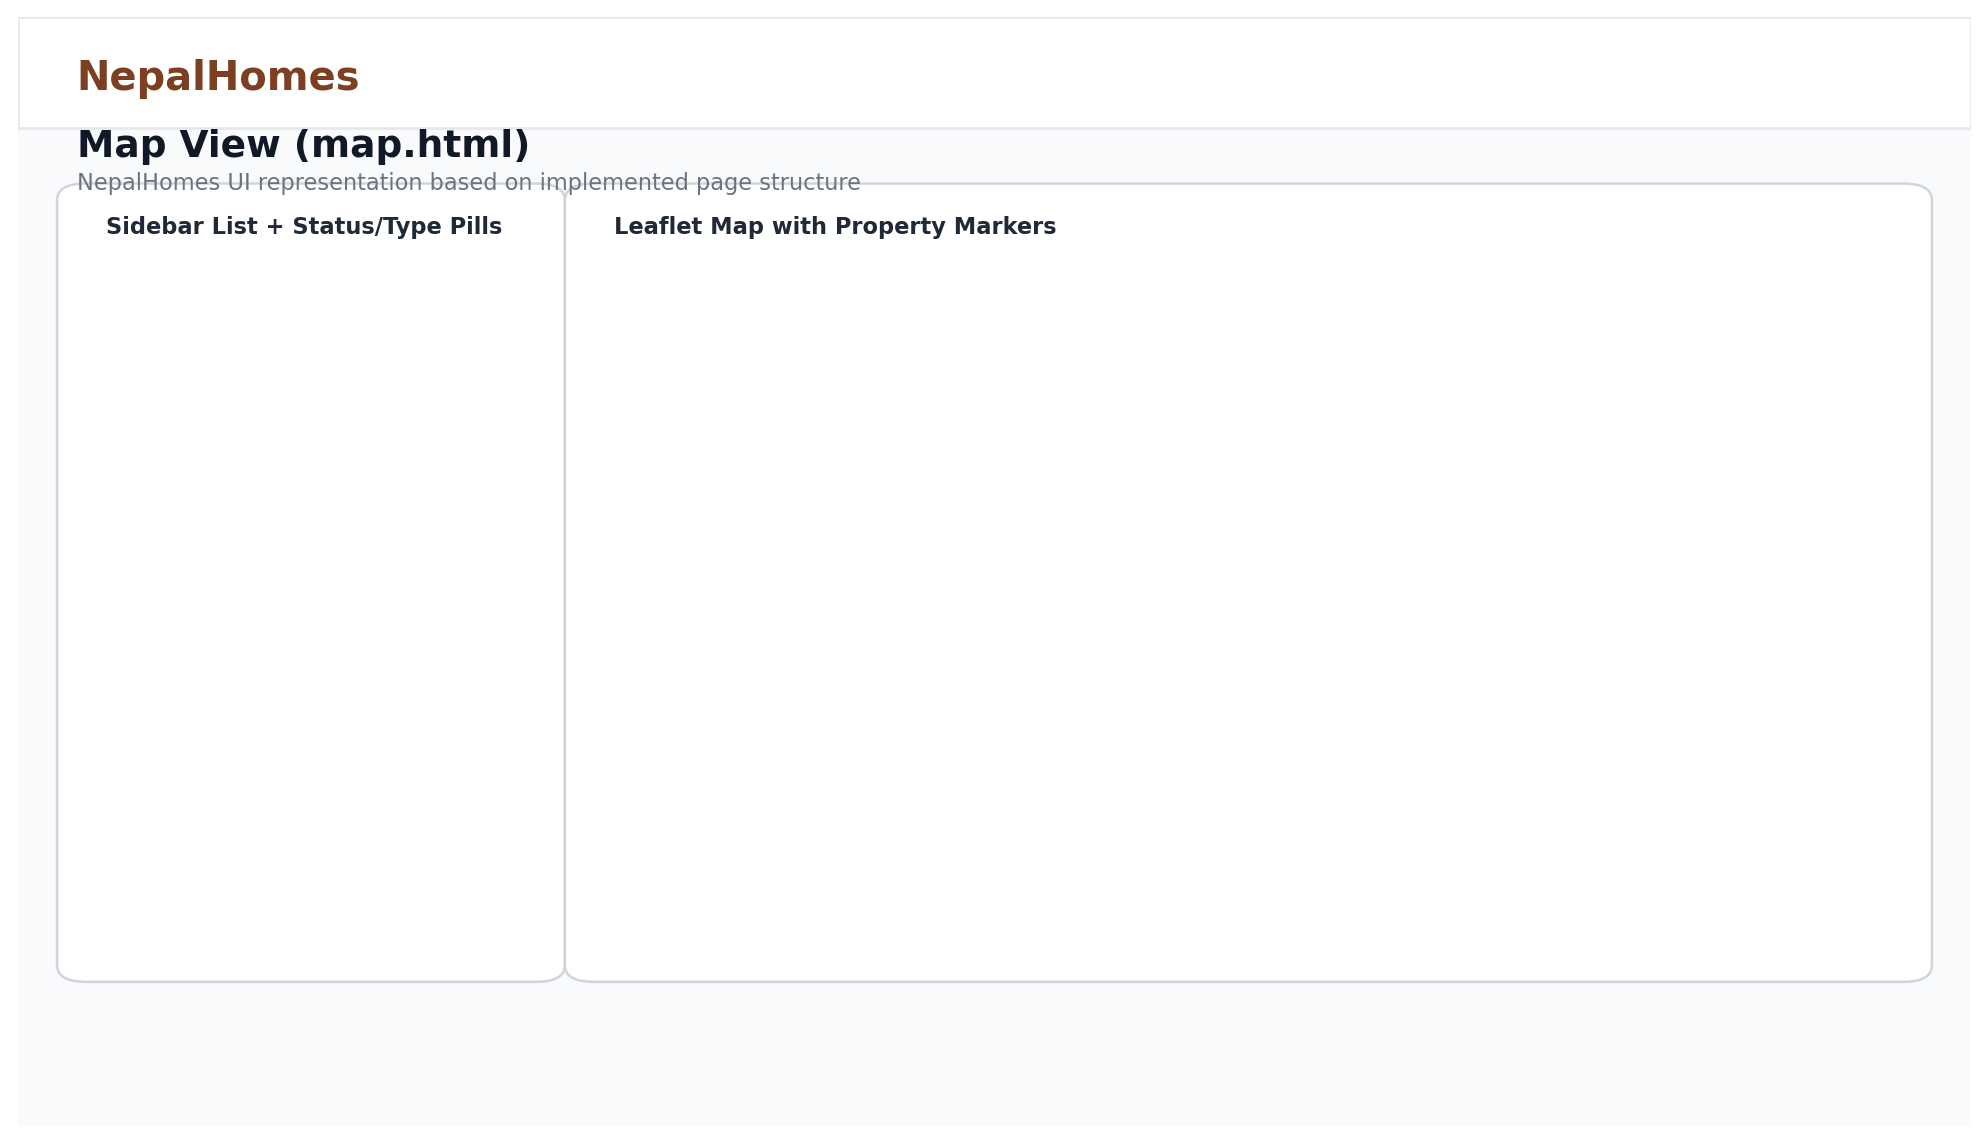
\includegraphics[width=0.95\textwidth]{figures/map_page.png}
    \vspace{1.2cm}}}
  \caption{Interactive Map View}
  \label{fig:map}
\end{figure}

\begin{figure}[H]
  \centering
  \fbox{\parbox{1\textwidth}{\centering\vspace{1.2cm}
    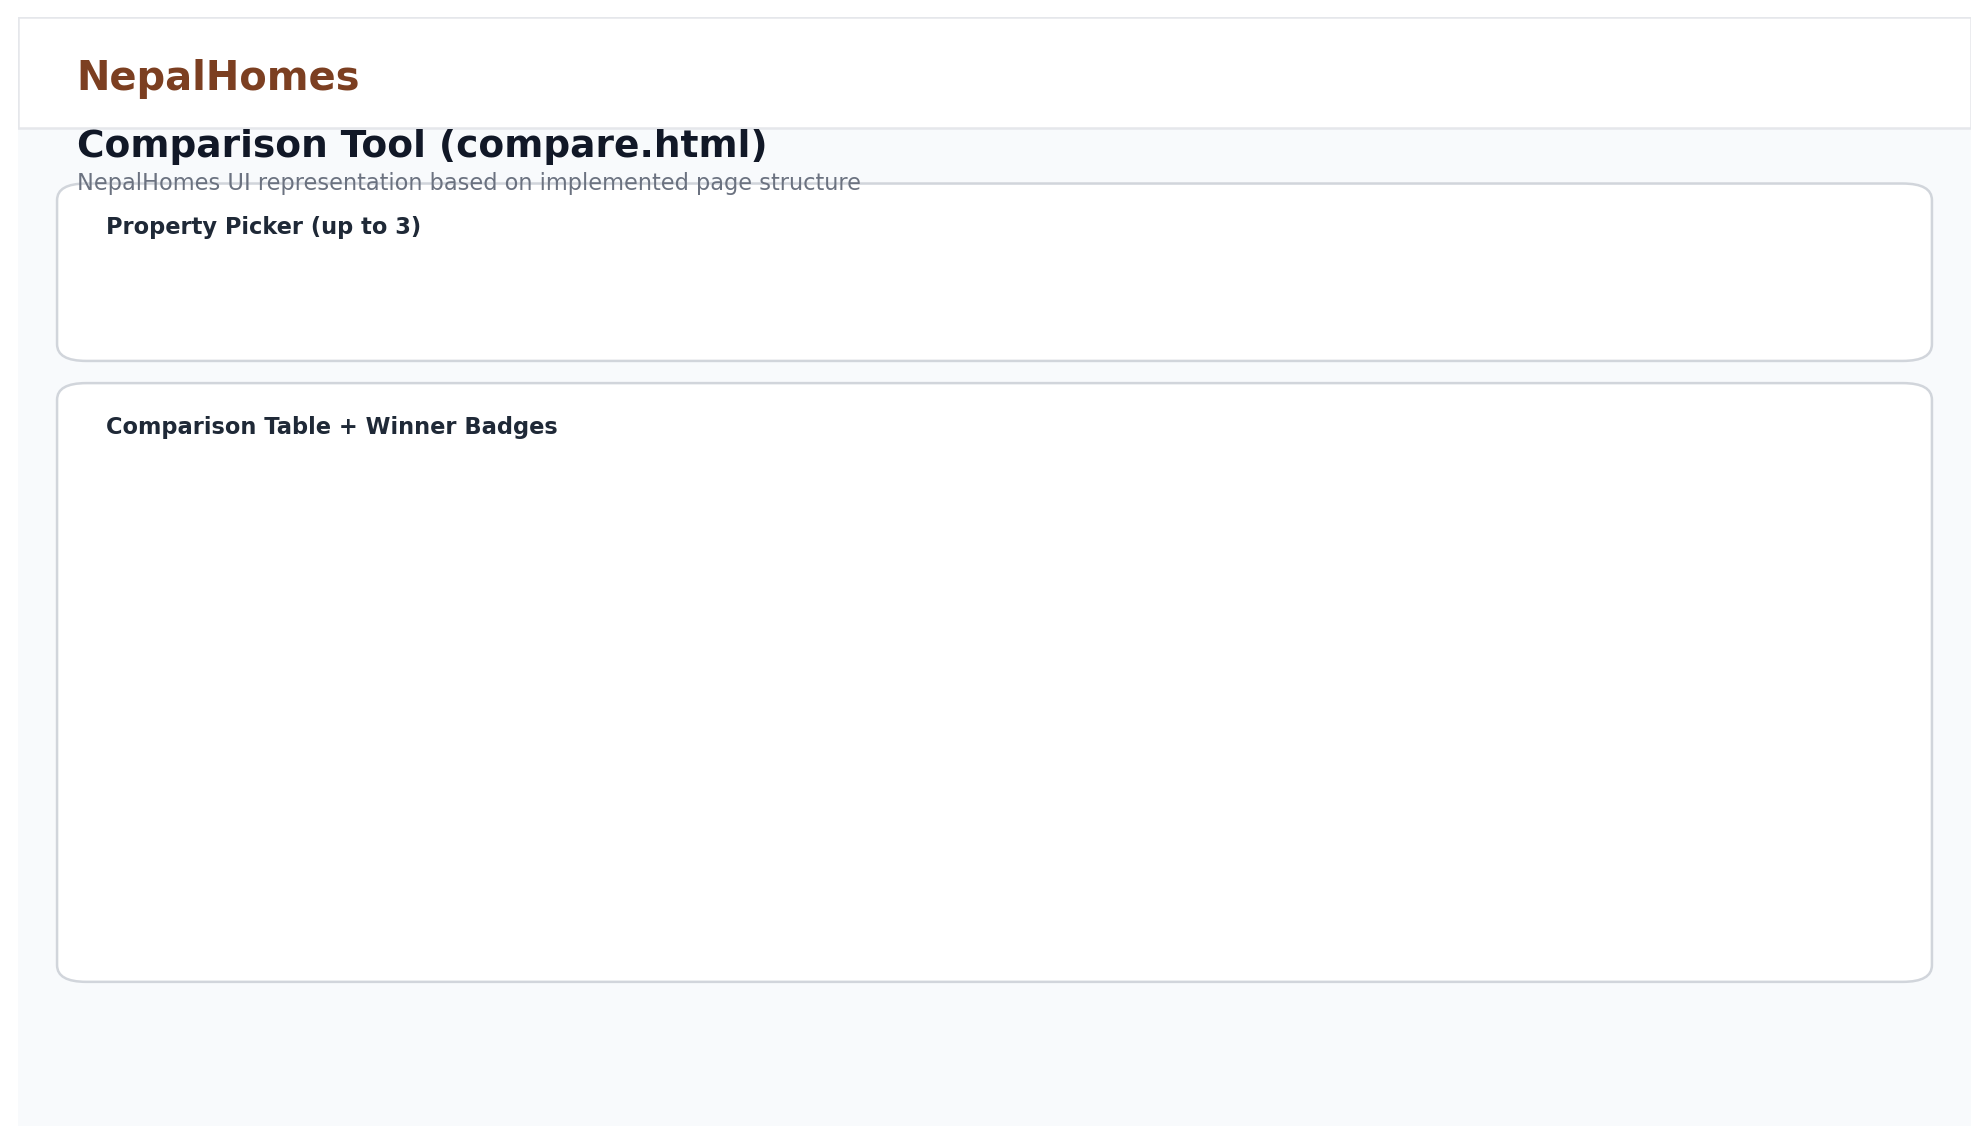
\includegraphics[width=0.95\textwidth]{figures/compare_page.png}
    \vspace{1.2cm}}}
  \caption{Property Comparison Tool}
  \label{fig:compare}
\end{figure}

\begin{figure}[H]
  \centering
  \fbox{\parbox{1\textwidth}{\centering\vspace{1.2cm}
    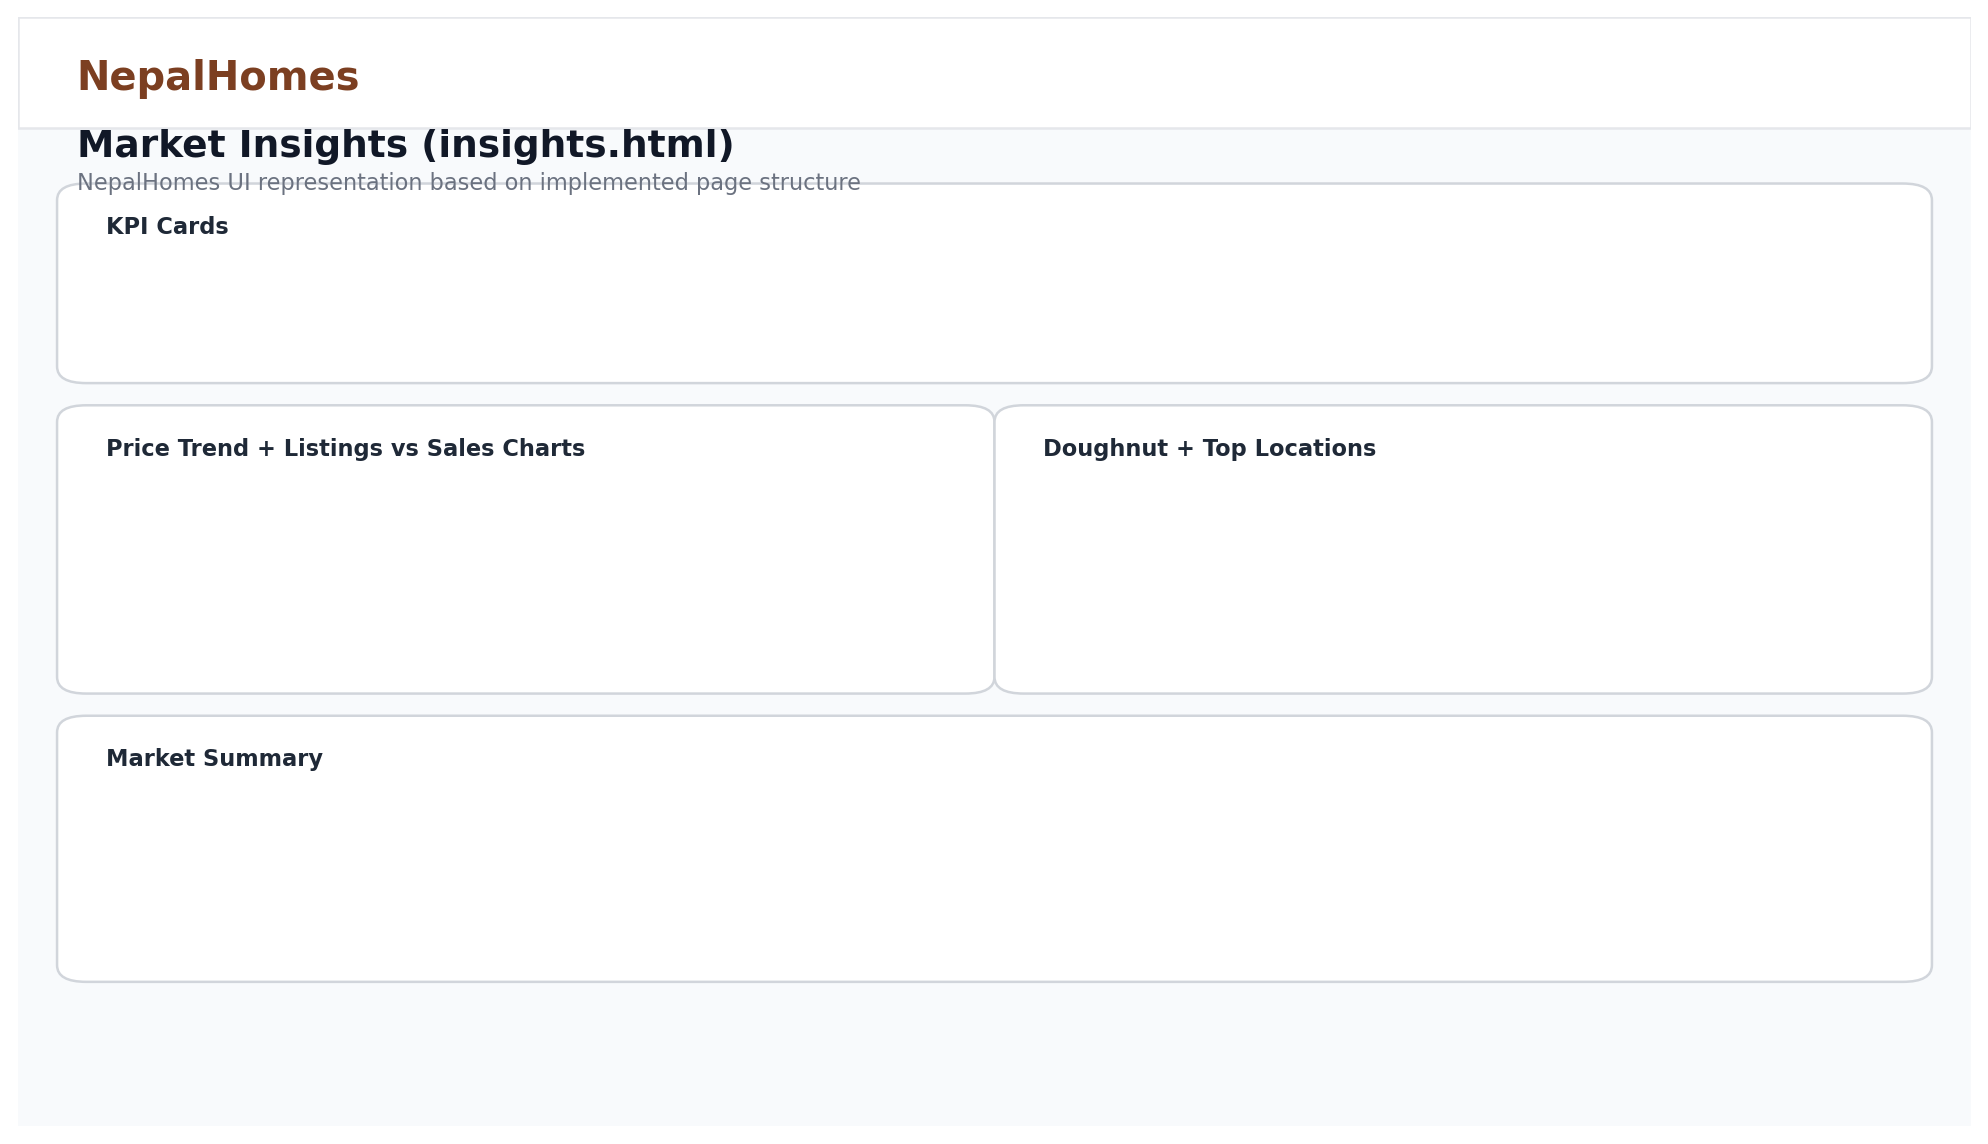
\includegraphics[width=0.95\textwidth]{figures/insights_page.png}
    \vspace{1.2cm}}}
  \caption{Market Insights Page with Chart.js Visualisations}
  \label{fig:insights}
\end{figure}

\begin{figure}[H]
  \centering
  \fbox{\parbox{1\textwidth}{\centering\vspace{1.2cm}
    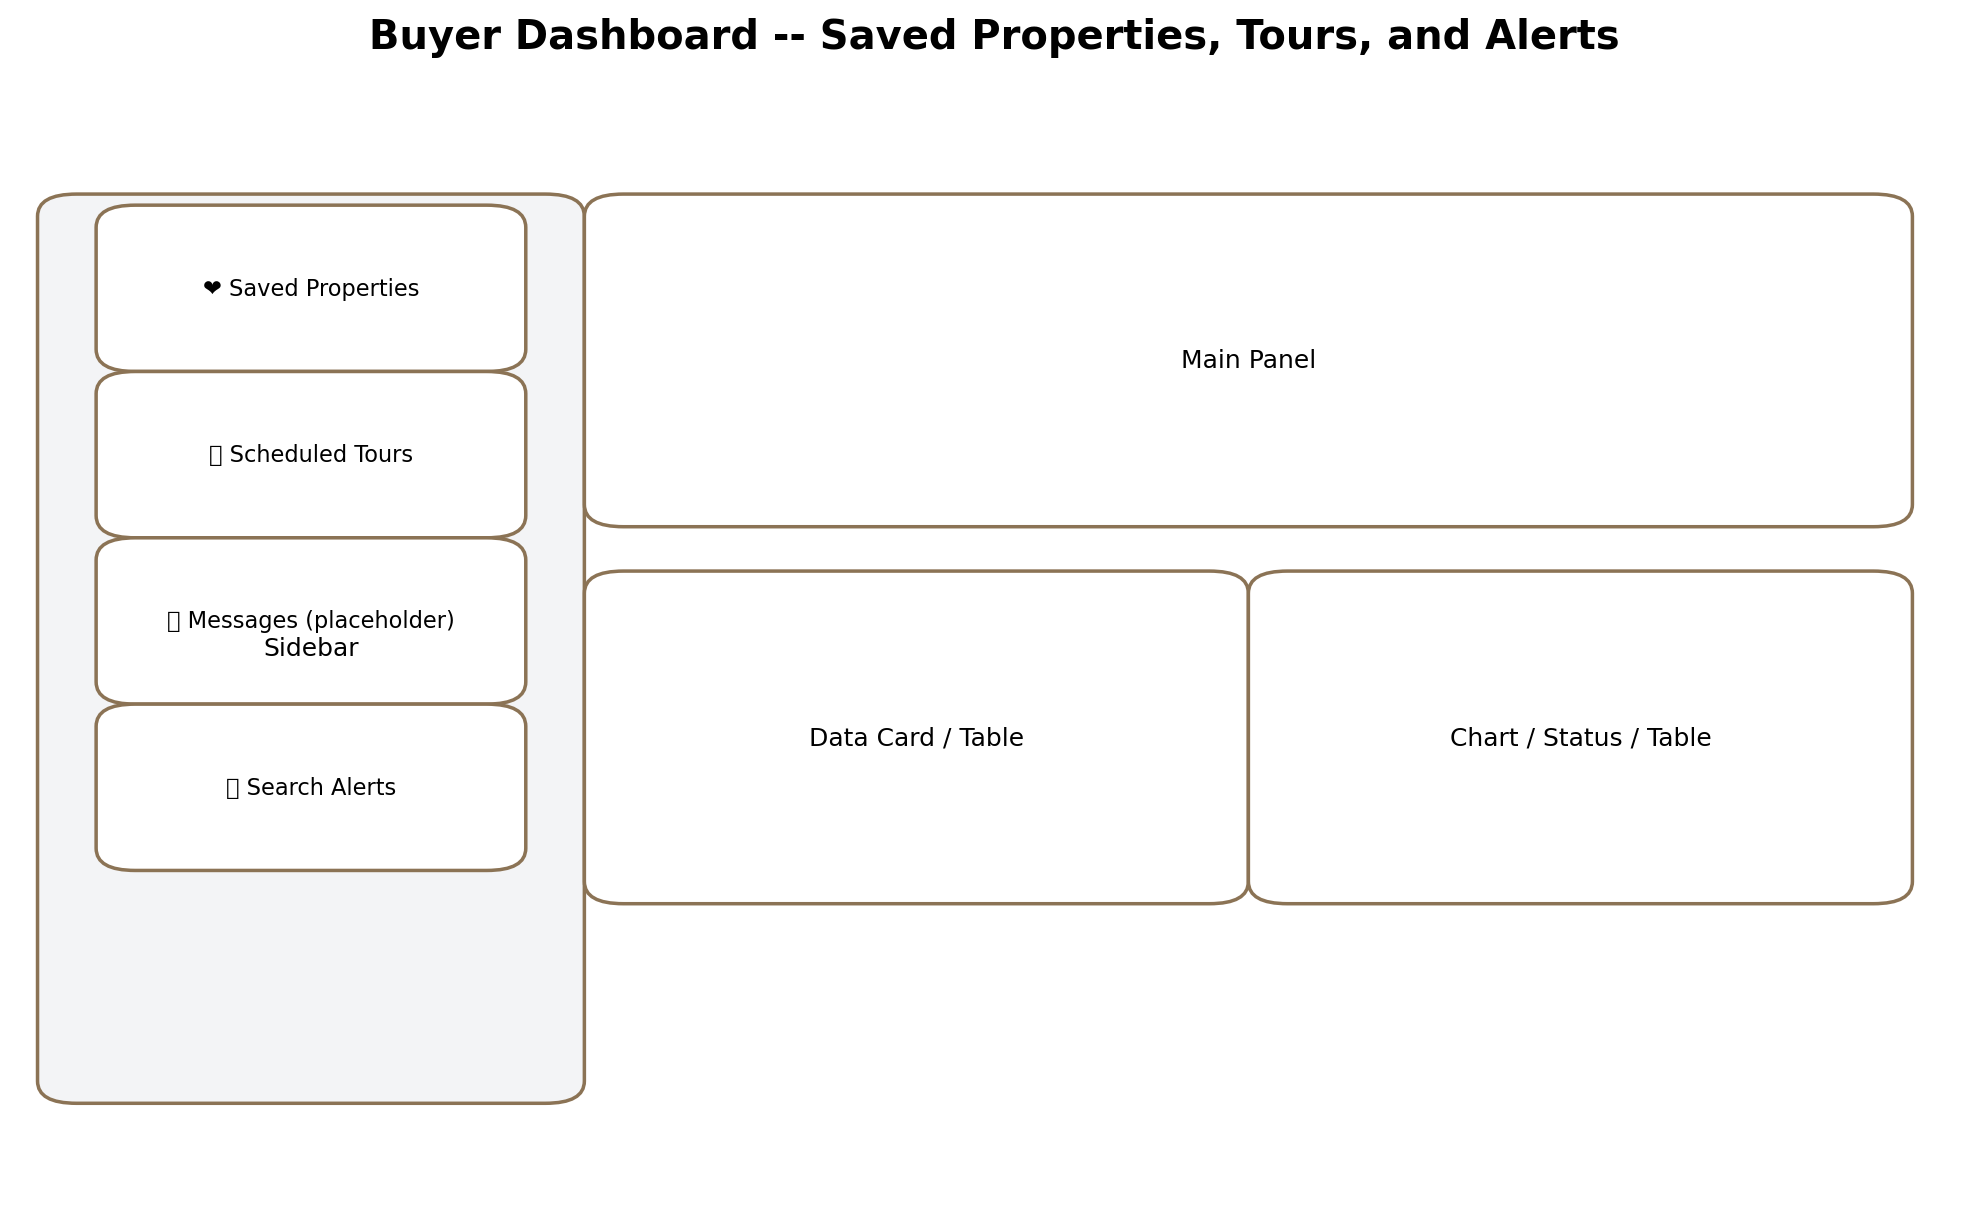
\includegraphics[width=0.95\textwidth]{figures/buyer_dashboard_mock.png}
    \vspace{1.2cm}}}
  \caption{Buyer Dashboard -- Saved Properties, Tours, and Alerts}
  \label{fig:buyer-dash}
\end{figure}

\begin{figure}[H]
  \centering
  \fbox{\parbox{1\textwidth}{\centering\vspace{1.2cm}
    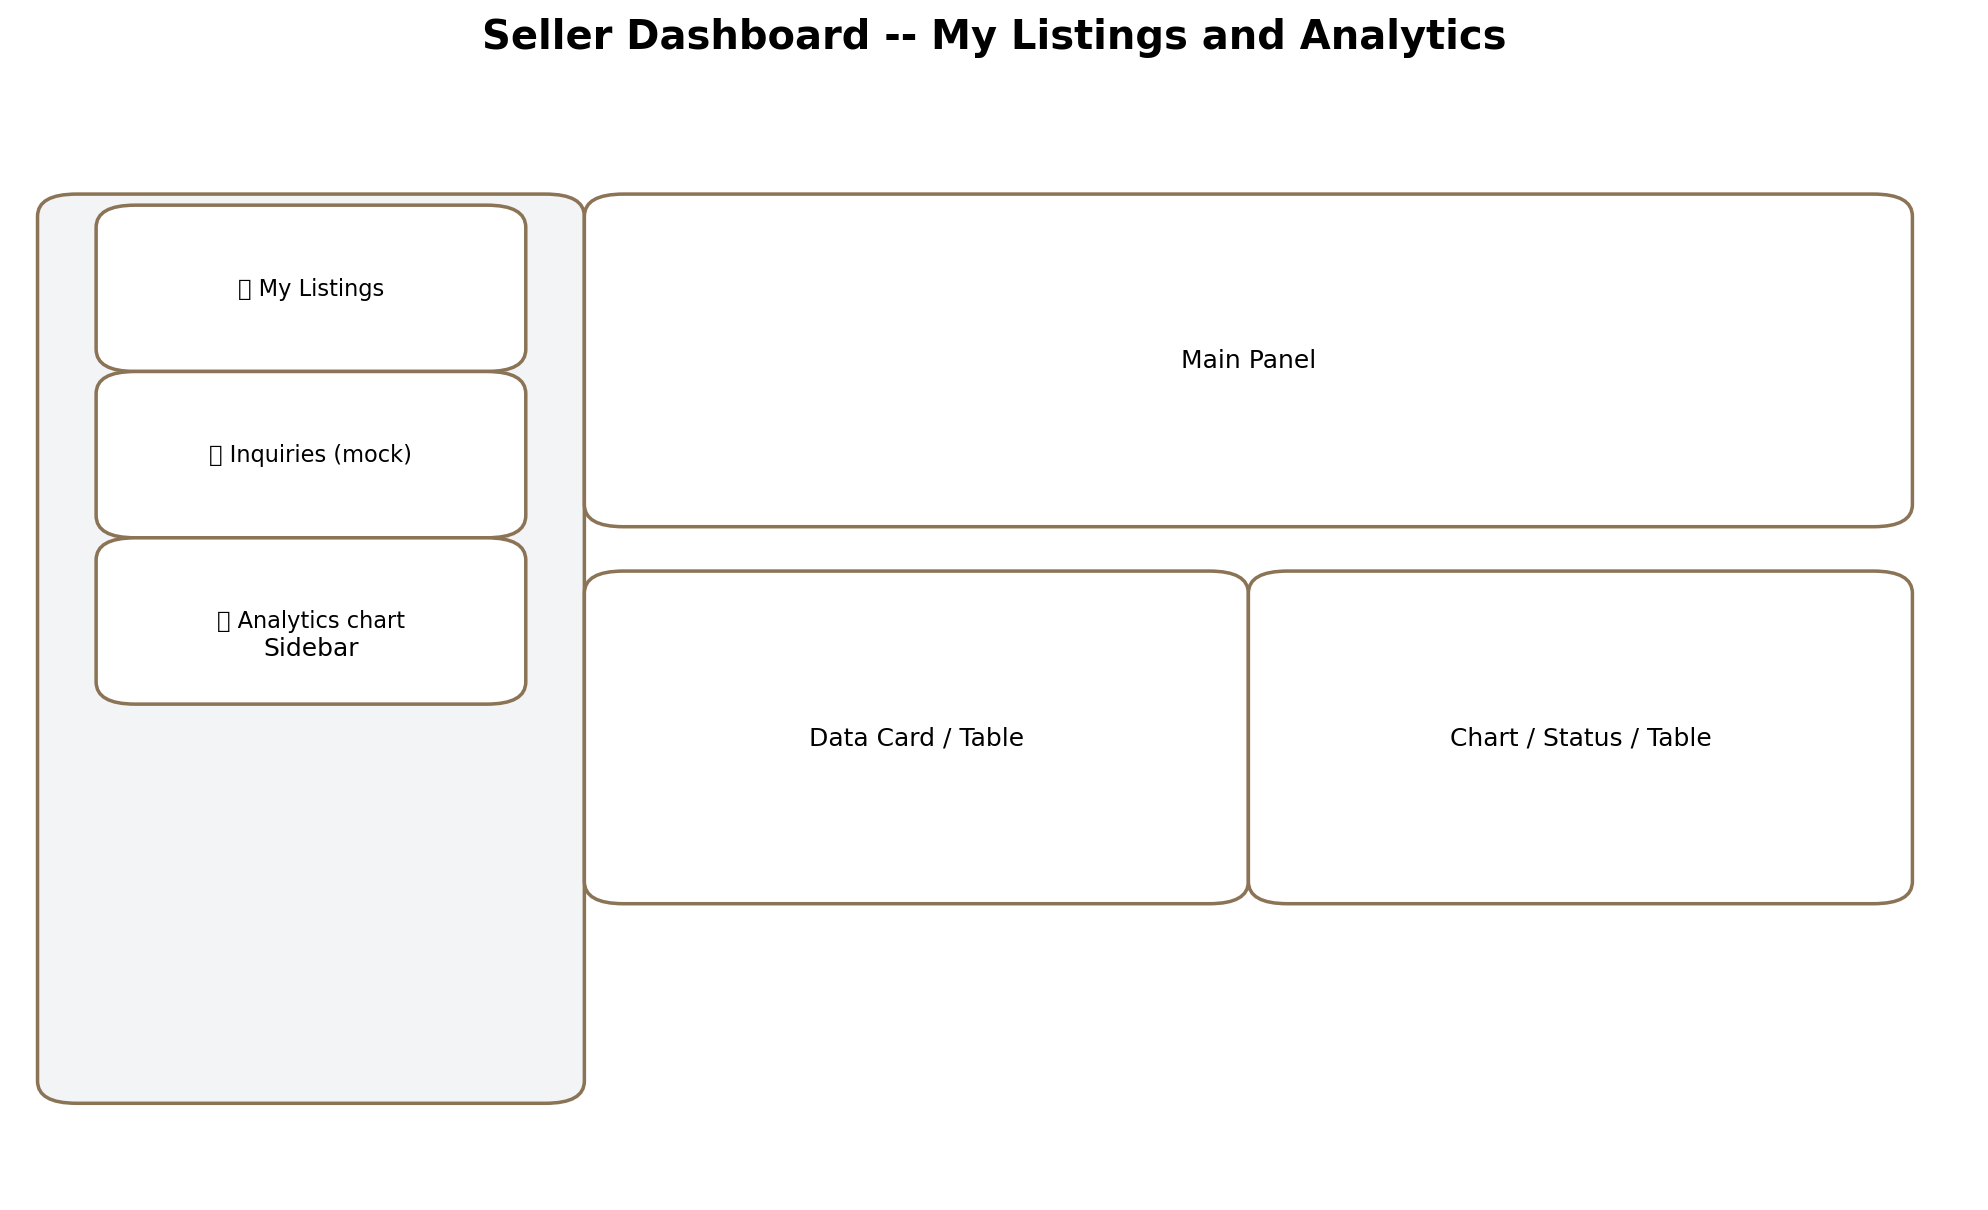
\includegraphics[width=0.95\textwidth]{figures/seller_dashboard_mock.png}
    \vspace{1.2cm}}}
  \caption{Seller Dashboard -- My Listings and Analytics}
  \label{fig:seller-dash}
\end{figure}

\begin{figure}[H]
  \centering
  \fbox{\parbox{1\textwidth}{\centering\vspace{1.2cm}
    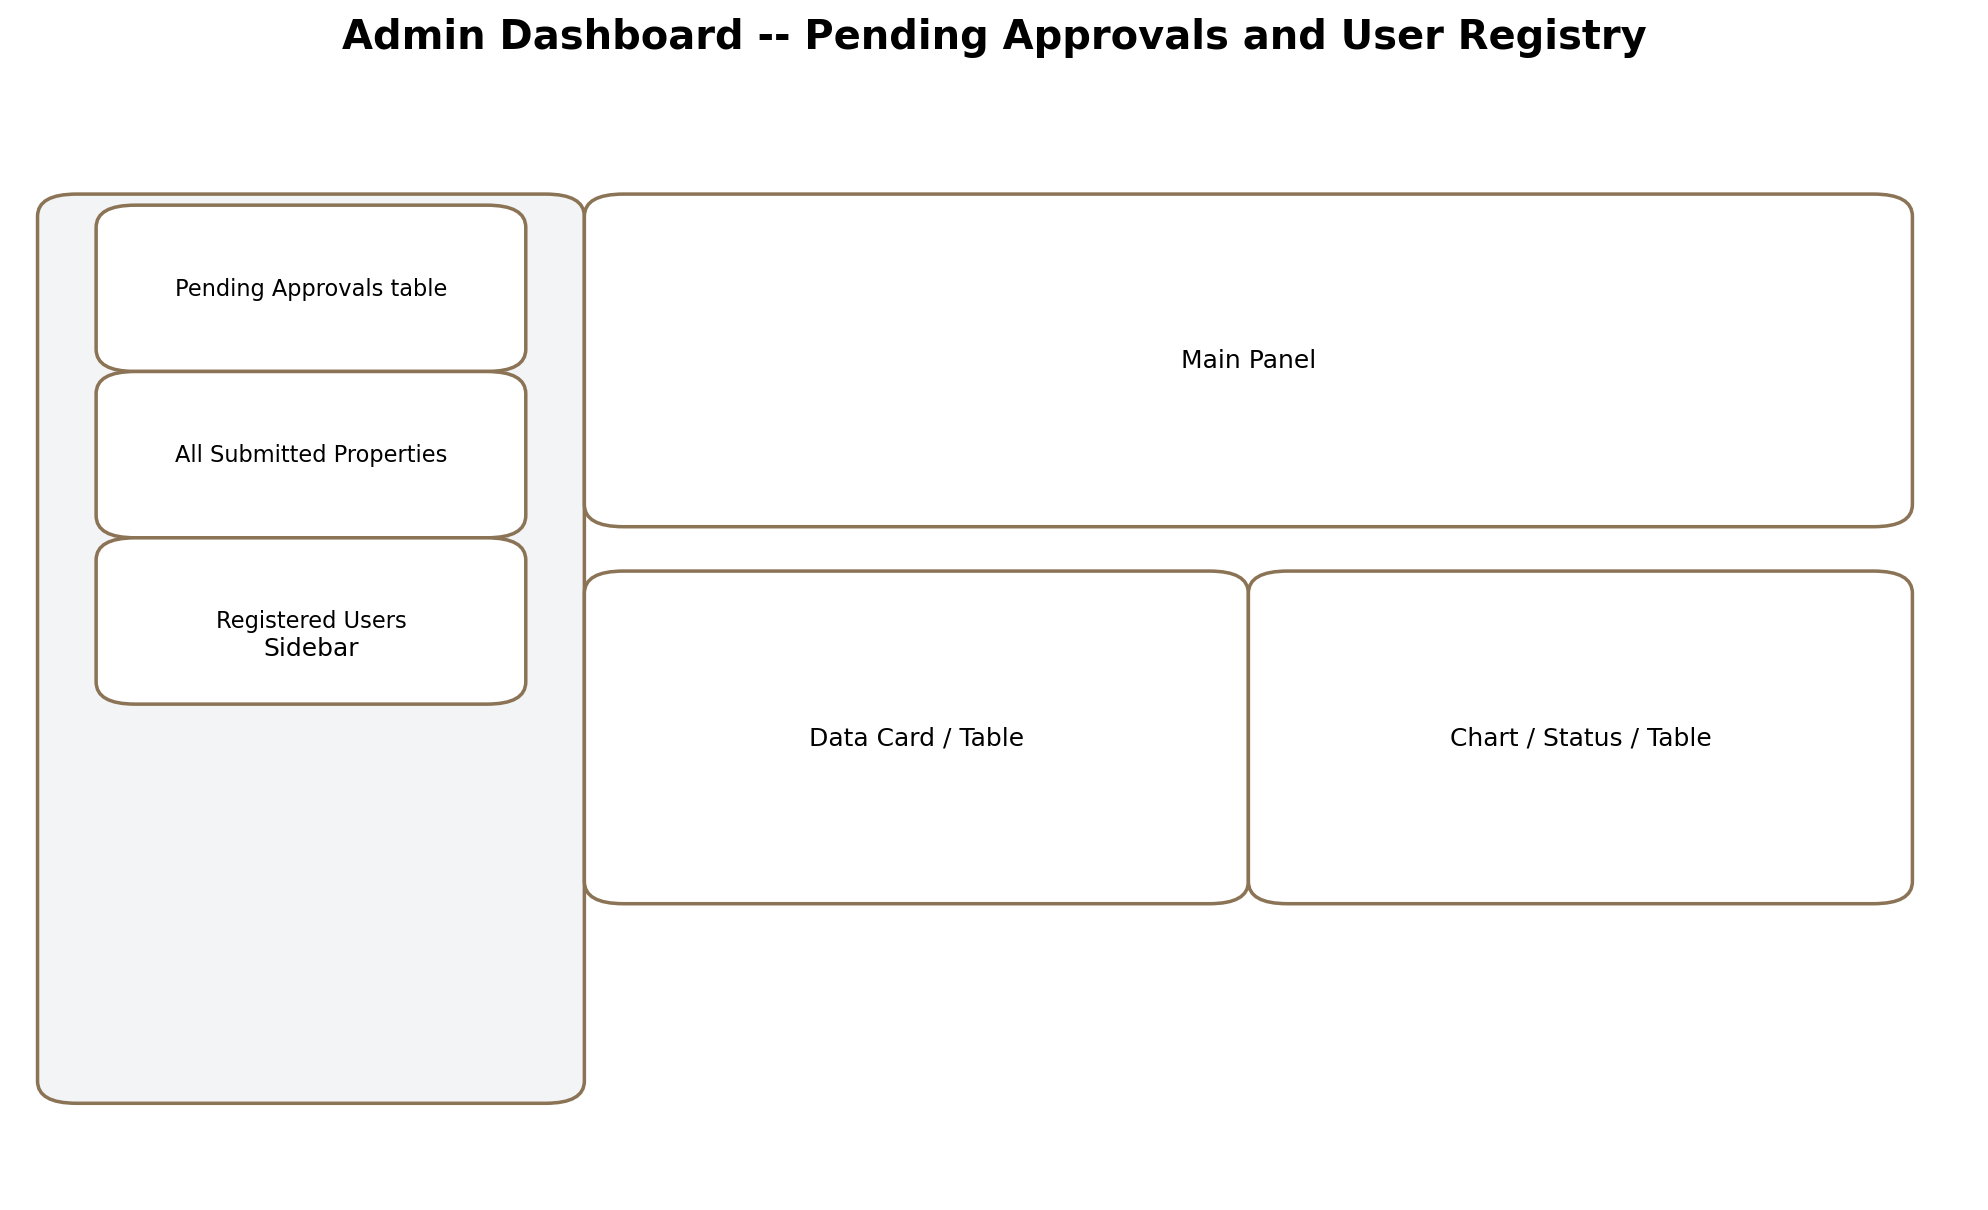
\includegraphics[width=0.95\textwidth]{figures/admin_dashboard_mock.png}
    \vspace{1.2cm}}}
  \caption{Admin Dashboard -- Pending Approvals and User Registry}
  \label{fig:admin-dash}
\end{figure}

%============================================================
\end{document}
%============================================================
